% =====================================================================
%  Hybrid Image Security -- draft v2 (revised after supervisor feedback)
%  Source of every number: the Hybrid-Image-Security repository
%  (paper/out/*.csv, paper/final/tables/*, paper/base_paper.py). Figures: paper/final/.
%  Compile from paper/manuscript/:  pdflatex main && pdflatex main
% =====================================================================
\documentclass[11pt,a4paper]{article}

\usepackage[utf8]{inputenc}
\IfFileExists{lmodern.sty}{\usepackage[T1]{fontenc}\usepackage{lmodern}}{} % falls back to Computer Modern
\usepackage[margin=2.2cm]{geometry}
\usepackage{amsmath,amssymb}
\usepackage{graphicx}
\usepackage{booktabs}
\usepackage{multirow}
\usepackage{array}
\usepackage{tabularx}
\usepackage{algorithm}
\usepackage{algpseudocode}
\usepackage{tikz}
\usetikzlibrary{positioning,arrows.meta,shapes.geometric,fit,calc}
\usepackage{xcolor}
\usepackage{caption}
\usepackage{enumitem}
\usepackage[section]{placeins}
\usepackage[hidelinks]{hyperref}

\graphicspath{{../final/}{figures/}}
\captionsetup{font=small,labelfont=bf}
\setlist{nosep,leftmargin=*}
\renewcommand{\arraystretch}{1.15}
\newcommand{\todo}[1]{\textcolor{red}{[#1]}}
\algrenewcommand\algorithmicrequire{\textbf{Input:}}
\algrenewcommand\algorithmicensure{\textbf{Output:}}

\title{Ownership-Safe Hybrid Image Security: Blind Block-SVD Watermarking with an RSA-Signed Certificate and an AES-256/RSA-2048 Hidden Channel}

\author{Nandika Agarwal\textsuperscript{1} \and Pranalee Patel\textsuperscript{1}\\[4pt]
\small\textsuperscript{1}NIIT University, Neemrana, India\\
\small Supervisor: \todo{Professor's name}, Cryptography course\\
\small\texttt{\todo{email addresses}}}
% TODO: confirm affiliation wording and the supervisor's name.

\date{Draft 2 --- November 2026}

\begin{document}
\maketitle

% =====================================================================
\begin{abstract}
\sloppy\noindent\textbf{In this article.}
QR-code watermarking in the DWT--SVD domain protects image ownership, but the base scheme reads its watermark using matrices supplied by the person making the claim, so an attacker can extract their own QR code from someone else's image. We propose a hybrid scheme for $512\times512$ colour images. A blind watermark in the blue channel stores the owner's QR code in the singular values of image blocks and is bound to the owner by an RSA-signed certificate. An AES-256 encrypted message, whose key is protected with RSA-2048, is hidden in the green channel.

\smallskip\noindent\textbf{Results.}
On 12 test images the protected image keeps a PSNR of 40.19\,dB while carrying both layers. False ownership claims are accepted on 0 of 12 images, against 12 of 12 for the base scheme. Under 11 attacks the watermark is read correctly in 103 of 132 cases, against 79, including all 12 images after JPEG compression at quality 50, where the base scheme manages 8. The hidden message is always recovered from an unmodified image. The scheme is weaker than the base scheme under heavy noise.

\smallskip\noindent\textbf{Improvement percentage.}
Against the base scheme under identical conditions: false-ownership acceptance improves by 100\%, correctly read attack cases by 30.4\%, NCC after blurring by 63.3\% and after rescaling by 65.1\%, and the verifier's key material shrinks by 99.96\%. Against the values reported in the base paper: NCC after JPEG compression improves by 0.65\%, while PSNR is 5.32\% lower.
% Formulas used (supervisor's definition): lower-is-better metrics (false acceptance, key material)
% Imp = (Old - New)/Old x 100; higher-is-better metrics (PSNR, NCC, read cases) Imp = (New - Old)/Old x 100.
% Comparison with 2-3 similar papers to be added once they are selected.
\end{abstract}

\smallskip\noindent\textbf{Keywords:} digital watermarking; QR code; DWT; SVD; quantisation index modulation; RSA; AES; steganography; ownership verification.

% =====================================================================
\section{Introduction}\label{sec:intro}

Digital images are copied and redistributed with little effort, so their owners need ways to prove ownership and, at times, to send confidential information inside the image itself~\cite{sanivarapu2022}. Encryption keeps content secret but makes it visibly protected. Steganography hides that a message exists but does not prove ownership. Watermarking embeds an identifier that survives ordinary processing and so supports ownership claims. This work combines all three in one colour image and, in doing so, repairs a security flaw in the watermarking scheme it builds on.

\subsection{Transform-domain watermarking with singular values}\label{sec:intro-core}

A watermark is embedded in a transform domain so that it spreads over many pixels and survives compression and filtering. The base paper~\cite{sanivarapu2022} applies a one-level discrete wavelet transform (DWT) to the blue channel of a $512\times512$ colour image and modifies the singular values of the $256\times256$ low-frequency (LL) sub-band, obtained by singular value decomposition (SVD). The LL band holds most of the image energy, and its singular values change little under small distortions~\cite{liu2002svd}. The watermark is a QR code of the owner's identity, scrambled with a chaotic logistic map~\cite{may1976} so that local damage spreads over the whole code.

We keep the DWT--SVD carrier but change how the watermark is written and read. Each QR bit is written into the largest singular value of one $8\times8$ block of the LL band (covering $16\times16$ image pixels) by quantisation index modulation (QIM). The value is moved to the centre of one of two interleaved quantisation cells, one for bit 0 and one for bit 1, as Figure~\ref{fig:qim-concept} shows. % CITATION NEEDED: QIM (e.g., Chen and Wornell, IEEE Trans. Inf. Theory, 2001)
The bit is read back from the image alone~\cite{TODO}. Ownership is then bound to the image by a certificate signed with RSA~\cite{rfc8017}, and a separate channel carries an AES-encrypted message~\cite{fips197}.

\begin{figure}[!htbp]
\centering
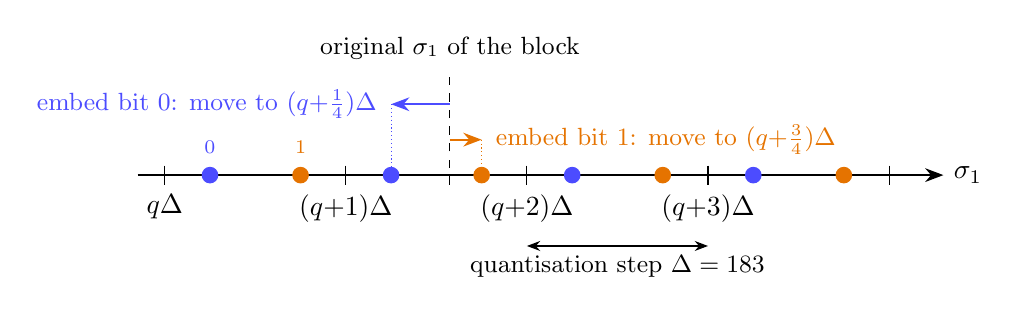
\begin{tikzpicture}[x=1.15cm,y=1cm,>=Stealth]
  \draw[->,thick] (-0.3,0) -- (8.6,0) node[right] {$\sigma_1$};
  \foreach \k in {0,2,4,6,8} {\draw (\k,0.12) -- (\k,-0.12);}
  \node[below] at (0,-0.12) {$q\Delta$};
  \node[below] at (2,-0.12) {$(q{+}1)\Delta$};
  \node[below] at (4,-0.12) {$(q{+}2)\Delta$};
  \node[below] at (6,-0.12) {$(q{+}3)\Delta$};
  \foreach \c in {0.5,2.5,4.5,6.5} {\fill[blue!70] (\c,0) circle (3pt);}
  \foreach \c in {1.5,3.5,5.5,7.5} {\fill[orange!90!black] (\c,0) circle (3pt);}
  \node[blue!70,above] at (0.5,0.15) {\scriptsize 0};
  \node[orange!90!black,above] at (1.5,0.15) {\scriptsize 1};
  \draw[dashed] (3.15,-0.12) -- (3.15,1.35) node[above,font=\small] {original $\sigma_1$ of the block};
  \draw[->,thick,orange!90!black] (3.15,0.45) -- (3.5,0.45);
  \node[orange!90!black,font=\small,anchor=west] at (3.55,0.45) {embed bit 1: move to $(q{+}\tfrac34)\Delta$};
  \draw[->,thick,blue!70] (3.15,0.9) -- (2.5,0.9);
  \node[blue!70,font=\small,anchor=east] at (2.45,0.9) {embed bit 0: move to $(q{+}\tfrac14)\Delta$};
  \draw[blue!70,densely dotted] (2.5,0.9) -- (2.5,0.08);
  \draw[orange!90!black,densely dotted] (3.5,0.45) -- (3.5,0.08);
  \draw[<->] (4,-0.9) -- (6,-0.9) node[midway,below,font=\small] {quantisation step $\Delta = 183$};
\end{tikzpicture}
\caption{\textbf{How one watermark bit is embedded (quantisation index modulation).} The horizontal axis is the largest singular value $\sigma_1$ of one $8\times8$ block of the LL band, divided into cells of width $\Delta$. Blue dots are the positions that encode bit 0, at $(q+\tfrac14)\Delta$; orange dots encode bit 1, at $(q+\tfrac34)\Delta$, where $q=\lfloor\sigma_1/\Delta\rfloor$. Embedding moves $\sigma_1$ to the nearest dot of the required colour; reading checks which colour $\sigma_1$ is closest to, using the received image only.}
\label{fig:qim-concept}
\end{figure}

\subsection{Why blind, certificate-bound embedding}\label{sec:intro-why}

The base scheme adds the watermark's singular values to the cover's and reconstructs the watermark from them using the QR code's own singular vectors, which the claimant keeps as a key. Those vectors carry most of the QR code's structure, so whoever supplies them largely decides what is extracted. Zhang and Li~\cite{zhang2005comments} pointed out this weakness in the scheme of Liu and Tan~\cite{liu2002svd}. Our reproduction shows that it is practical against the base scheme: an attacker's own vectors extract the attacker's QR code from the owner's image on all 12 test images (Section~\ref{sec:res-own}).

Signing the key file does not repair this, because an attacker can sign fake keys with their own RSA key. The repair must remove the claimant's influence over the extracted watermark. Blind QIM extraction does this: the bits come from the image, and the certificate only names the key and settings needed to read them. The RSA signature then ties the identity in the QR code to a public key. Dropping the cover image and the singular-vector matrices from the verifier's inputs also shrinks the key material from about 1.8\,MB to 758 bytes. The hidden message follows the standard hybrid pattern: AES-256~\cite{fips197} encrypts the data, and RSA-2048~\cite{rfc8017} protects the AES key.

\subsection{Existing work and contributions}\label{sec:intro-related}

Liu and Tan~\cite{liu2002svd} proposed modifying an image's singular values to carry a watermark for rightful-ownership protection, and Zhang and Li~\cite{zhang2005comments} showed that such schemes can return a watermark that was never embedded when the verifier uses singular vectors chosen by the claimant. Sanivarapu et al.~\cite{sanivarapu2022} combined a QR-code watermark, RSA, logistic-map scrambling and DWT--SVD embedding in the blue channel of $512\times512$ colour images, reporting a mean PSNR of 42.45\,dB on 12 images and NCC between 0.978 and 0.996 under eight attacks, but without testing false ownership claims or carrying a confidential payload. For hidden data, the SPAM features of Pevn\'y et al.~\cite{pevny2010spam} and the BOSS benchmark~\cite{bas2011boss} are the standard tools for testing detectability. % CITATION NEEDED: 2-3 similar papers to be added to this paragraph once selected.

The contributions of this work are:
\begin{itemize}
  \item A blind watermark that stores each QR bit in the singular values of image blocks, bound to the owner by an RSA-signed certificate. It rejects every false-ownership claim (0/12, against 12/12 for the base scheme) and needs no cover image to verify.
  \item A hybrid scheme for $512\times512$ colour images that combines this watermark with an AES-256/RSA-2048 encrypted message in a separate colour channel, at the same image quality as the base scheme (40.19 vs 40.12\,dB).
  \item A full evaluation against the reproduced base scheme under 11 attacks, with capacity, steganalysis and security tests, reporting both where the proposed scheme is better and where it is weaker.
\end{itemize}

Figure~\ref{fig:overview} gives an overview of the proposed system.

\begin{figure}[!htbp]
\centering
\resizebox{\textwidth}{!}{%
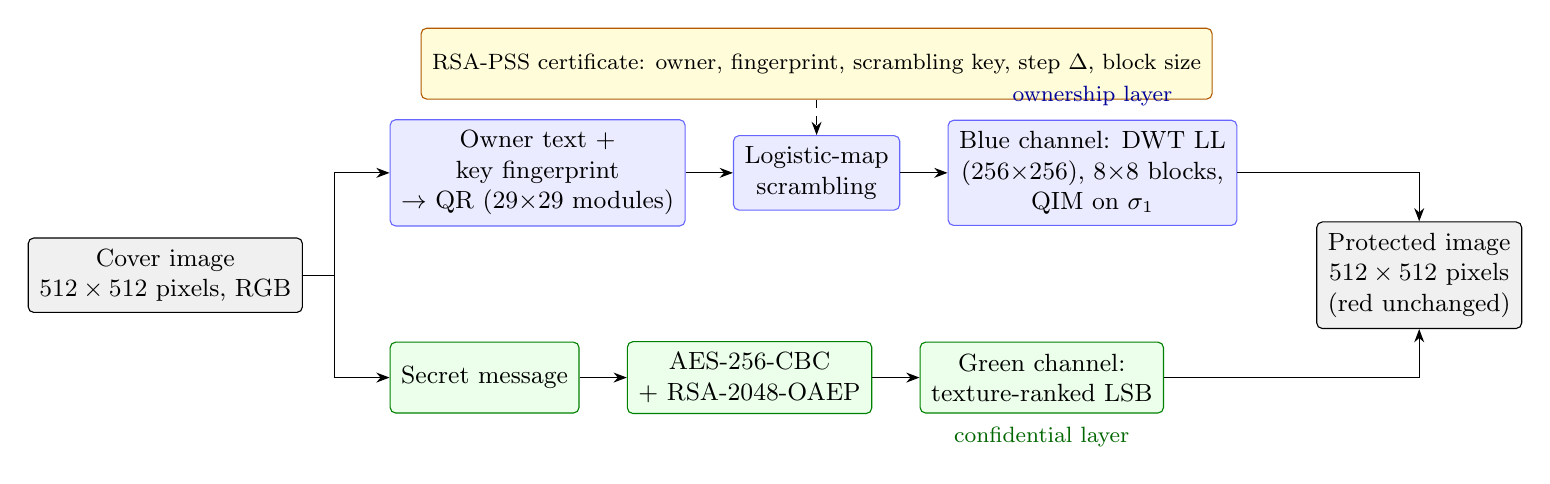
\begin{tikzpicture}[>=Stealth, node distance=0.5cm and 0.6cm,
  box/.style={draw, rounded corners=2pt, align=center, font=\small, minimum height=0.9cm, inner sep=4pt},
  img/.style={box, fill=gray!12},
  blue/.style={box, fill=blue!8, draw=blue!60},
  green/.style={box, fill=green!8, draw=green!50!black},
  key/.style={box, fill=yellow!15, draw=orange!70!black, font=\footnotesize}]
  \node[img] (cover) {Cover image\\$512\times512$ pixels, RGB};
  \node[blue, right=1.1cm of cover, yshift=1.3cm] (qr) {Owner text +\\key fingerprint\\$\rightarrow$ QR ($29{\times}29$ modules)};
  \node[blue, right=of qr] (scr) {Logistic-map\\scrambling};
  \node[blue, right=of scr] (qim) {Blue channel: DWT LL\\($256{\times}256$), $8{\times}8$ blocks,\\QIM on $\sigma_1$};
  \node[green, right=1.1cm of cover, yshift=-1.3cm] (msg) {Secret message};
  \node[green, right=of msg] (enc) {AES-256-CBC\\+ RSA-2048-OAEP};
  \node[green, right=of enc] (lsb) {Green channel:\\texture-ranked LSB};
  \node[img, right=1.0cm of qim, yshift=-1.3cm] (out) {Protected image\\$512\times512$ pixels\\(red unchanged)};
  \node[key, above=0.45cm of scr] (cert) {RSA-PSS certificate: owner, fingerprint, scrambling key, step $\Delta$, block size};
  \draw[->] (cover.east) -- ++(0.4,0) |- (qr.west);
  \draw[->] (cover.east) -- ++(0.4,0) |- (msg.west);
  \draw[->] (qr) -- (scr); \draw[->] (scr) -- (qim); \draw[->] (msg) -- (enc); \draw[->] (enc) -- (lsb);
  \draw[->] (qim.east) -| (out.north); \draw[->] (lsb.east) -| (out.south);
  \draw[->, dashed] (cert.south) -- (scr.north);
  \node[font=\footnotesize, blue!60!black, above=0.05cm of qim] {ownership layer};
  \node[font=\footnotesize, green!40!black, below=0.05cm of lsb] {confidential layer};
\end{tikzpicture}}
\caption{\textbf{Block diagram of the proposed hybrid image security system.} The upper path (blue) builds the ownership watermark: a QR code of the owner's name and key fingerprint is scrambled and embedded in the blue channel. The lower path (green) encrypts a secret message and hides it in the green channel. The two layers occupy different channels, so neither overwrites the other; the red channel is left unchanged. The signed certificate (yellow) records the settings needed to read the watermark.}
\label{fig:overview}
\end{figure}

\paragraph{Organisation.} Section~\ref{sec:alg} presents the DWT, SVD, RSA-2048 and AES-256 algorithms. Section~\ref{sec:method} describes the full pipeline, its parameters and the experimental setup. Section~\ref{sec:results} presents the results and compares them with the base paper. Section~\ref{sec:conclusion} concludes and outlines future work.

% =====================================================================
\section{Algorithm Details}\label{sec:alg}

This section gives the four algorithms the scheme is built on. DWT and SVD are used by the base paper~\cite{sanivarapu2022}; RSA-2048 and AES-256 are added in this work. Table~\ref{tab:notation} lists the notation.

\begin{table}[!htbp]
\centering\small
\caption{Notation.}\label{tab:notation}
\begin{tabularx}{\textwidth}{@{}lX@{}}
\toprule
Symbol & Meaning \\
\midrule
$I$; $I_R, I_G, I_B$ & Cover image ($512\times512$ pixels, 3 channels, 8 bits each); its red, green and blue channels \\
$X$ & One channel or sub-band processed by the DWT \\
$LL, LH, HL, HH$ & Approximation and detail sub-bands of the one-level 2-D Haar DWT ($256\times256$ each) \\
$A = U\Sigma V^{\top}$ & Singular value decomposition of a matrix $A$; $U,V$ orthonormal, $\Sigma=\mathrm{diag}(\sigma_1\ge\sigma_2\ge\dots\ge0)$ \\
$\lambda_i$, $\mathbf{v}_i$, $\mathbf{u}_i$ & Eigenvalues and eigenvectors of $A^{\top}A$; left singular vectors \\
$\sigma_1$ & Largest singular value of an $8\times8$ LL block \\
$\Delta$, $q$ & QIM step (183) and cell index $\lfloor\sigma_1/\Delta\rfloor$ \\
$r$, $x_0$ & Logistic-map parameter and initial value (scrambling key) \\
$p, q_{\mathrm{rsa}}, n$ & RSA primes (1024 bits each) and modulus $n=p\,q_{\mathrm{rsa}}$ (2048 bits) \\
$e$, $d$, $\lambda(n)$ & RSA public exponent (65537), private exponent, Carmichael function of $n$ \\
$K_{pub}$, $K_{priv}$ & RSA public key $(n,e)$ and private key $(n,d)$ \\
$H(\cdot)$ & SHA-256 hash \\
$m$, $c$, $s$ & RSA message representative, ciphertext and signature \\
$K_{AES}$, $IV$ & 256-bit AES key and 128-bit initialisation vector \\
$P_i$, $C_i$ & $i$-th 16-byte plaintext and ciphertext block; $C_0 = IV$ \\
$\mathrm{AES}_K$, $\mathrm{AES}_K^{-1}$ & AES block encryption and decryption under key $K$ (14 rounds) \\
\bottomrule
\end{tabularx}
\end{table}

\subsection{Discrete wavelet transform}

The one-level 2-D Haar DWT splits a channel into four half-size sub-bands. With the orthonormal Haar filters, every $2\times2$ pixel group maps to one coefficient in each sub-band (Algorithm~\ref{alg:dwt}), and the transform is exactly invertible. For a $512\times512$ channel each sub-band is $256\times256$. % CITATION NEEDED: wavelet transform (e.g., Mallat 1989)

\begin{algorithm}[!htbp]
\caption{One-level 2-D Haar DWT and its inverse}\label{alg:dwt}
\begin{algorithmic}[1]
\Require channel $X$ of size $2m\times2m$ (here $512\times512$)
\Ensure sub-bands $LL, LH, HL, HH$ of size $m\times m$ (here $256\times256$)
\For{$i \gets 0$ \textbf{to} $m-1$, $j \gets 0$ \textbf{to} $m-1$}
  \State $a\gets X_{2i,2j}$, $b\gets X_{2i,2j+1}$, $c\gets X_{2i+1,2j}$, $g\gets X_{2i+1,2j+1}$
  \State $LL_{ij}\gets (a+b+c+g)/2$; \quad $LH_{ij}\gets (a+b-c-g)/2$
  \State $HL_{ij}\gets (a-b+c-g)/2$; \quad $HH_{ij}\gets (a-b-c+g)/2$
\EndFor
\State \textbf{Inverse:} $a=(LL+LH+HL+HH)/2$, $b=(LL+LH-HL-HH)/2$, $c=(LL-LH+HL-HH)/2$, $g=(LL-LH-HL+HH)/2$
\State \Return $LL, LH, HL, HH$ \Comment{sign conventions of the detail bands follow PyWavelets}
\end{algorithmic}
\end{algorithm}

\subsection{Singular value decomposition}

Any real matrix $A$ factors as $A=U\Sigma V^{\top}$ with orthonormal $U,V$ and non-negative singular values on the diagonal of $\Sigma$. The largest singular value $\sigma_1$ measures the energy of the block's dominant pattern and changes little under small distortions. Algorithm~\ref{alg:svd} states the decomposition through the eigen-decomposition of $A^{\top}A$; the implementation calls the LAPACK routine behind \texttt{numpy.linalg.svd}.

\begin{algorithm}[!htbp]
\caption{Singular value decomposition (conceptual)}\label{alg:svd}
\begin{algorithmic}[1]
\Require matrix $A\in\mathbb{R}^{k\times k}$ (here an $8\times8$ LL block)
\Ensure $U, \Sigma, V$ with $A=U\Sigma V^{\top}$
\State compute the eigenpairs $(\lambda_i, \mathbf{v}_i)$ of $A^{\top}A$, sorted so that $\lambda_1\ge\lambda_2\ge\dots\ge0$
\For{$i\gets1$ \textbf{to} $k$}
  \State $\sigma_i\gets\sqrt{\lambda_i}$
  \State $\mathbf{u}_i\gets A\mathbf{v}_i/\sigma_i$ \textbf{if} $\sigma_i>0$ \textbf{else} complete $U$ to an orthonormal basis
\EndFor
\State $U\gets[\mathbf{u}_1\dots\mathbf{u}_k]$, $\Sigma\gets\mathrm{diag}(\sigma_1,\dots,\sigma_k)$, $V\gets[\mathbf{v}_1\dots\mathbf{v}_k]$
\State \Return $U,\Sigma,V$
\end{algorithmic}
\end{algorithm}

\subsection{RSA-2048}

RSA~\cite{rfc8017} is used twice: to wrap the AES key of the hidden message (OAEP padding), and to sign the ownership certificate (PSS padding). Algorithm~\ref{alg:rsa} summarises key generation and both uses; the padding schemes follow PKCS\#1 v2.2~\cite{rfc8017} as implemented in PyCryptodome.

\begin{algorithm}[!htbp]
\caption{RSA-2048: key generation, OAEP key wrapping and PSS signatures}\label{alg:rsa}
\begin{algorithmic}[1]
\Require key size 2048 bits; AES key to wrap; document to sign
\Ensure $(K_{pub},K_{priv})$; wrapped key $c$; signature $s$
\State choose random primes $p, q_{\mathrm{rsa}}$ of 1024 bits; $n\gets p\,q_{\mathrm{rsa}}$; $\lambda(n)\gets\mathrm{lcm}(p-1,q_{\mathrm{rsa}}-1)$
\State $e\gets65537$; \quad $d\gets e^{-1}\bmod\lambda(n)$; \quad $K_{pub}\gets(n,e)$, $K_{priv}\gets(n,d)$
\State \textbf{OAEP wrap:} $m\gets\mathrm{OAEP\text{-}encode}(K_{AES})$; \quad $c\gets m^{e}\bmod n$ \Comment{256-byte block}
\State \textbf{OAEP unwrap:} $m\gets c^{d}\bmod n$; \quad $K_{AES}\gets\mathrm{OAEP\text{-}decode}(m)$
\State \textbf{PSS sign:} $m\gets\mathrm{PSS\text{-}encode}(H(\text{document}))$; \quad $s\gets m^{d}\bmod n$
\State \textbf{PSS verify:} $m\gets s^{e}\bmod n$; \quad accept iff $\mathrm{PSS\text{-}verify}(m, H(\text{document}))$
\end{algorithmic}
\end{algorithm}

\subsection{AES-256}

The secret message is encrypted with AES~\cite{fips197} under a fresh random 256-bit key and 128-bit IV, in cipher-block-chaining (CBC) mode with PKCS\#7 padding (Algorithm~\ref{alg:aes}). % CITATION NEEDED: CBC mode (NIST SP 800-38A)
CBC makes each ciphertext block depend on all earlier plaintext blocks~\cite{TODO}.

\begin{algorithm}[!htbp]
\caption{AES-256-CBC encryption and decryption}\label{alg:aes}
\begin{algorithmic}[1]
\Require plaintext bytes; for decryption, $K_{AES}$, $IV$ and the ciphertext
\Ensure $(K_{AES}, IV, C_1\|\dots\|C_t)$; recovered plaintext
\State $K_{AES}\gets$ 32 random bytes; \quad $IV\gets$ 16 random bytes
\State pad the plaintext with PKCS\#7 to a multiple of 16 bytes; split into blocks $P_1,\dots,P_t$
\State expand $K_{AES}$ into 15 round keys \Comment{14 rounds for a 256-bit key}
\State $C_0\gets IV$
\For{$i\gets1$ \textbf{to} $t$}
  \State $C_i\gets\mathrm{AES}_{K}(P_i\oplus C_{i-1})$ \Comment{SubBytes, ShiftRows, MixColumns, AddRoundKey}
\EndFor
\State \textbf{Decrypt:} $P_i\gets\mathrm{AES}^{-1}_{K}(C_i)\oplus C_{i-1}$ for $i=1..t$; remove the padding
\State \Return $(K_{AES}, IV, C_1\|\dots\|C_t)$
\end{algorithmic}
\end{algorithm}

% =====================================================================
\section{Methodology}\label{sec:method}

The proposed system protects a $512\times512$-pixel colour image with two independent layers. This section describes each step, then explains the flowchart of Figure~\ref{fig:flow}.

\subsection{Ownership layer (blue channel)}

\paragraph{Watermark.} The owner's RSA public key is hashed with SHA-256, and its first eight hexadecimal digits form a fingerprint. The text ``owner name $|$ pk:fingerprint'' is encoded as a QR code with error-correction level H, giving a grid of $29\times29=841$ modules.

\paragraph{Scrambling.} The logistic map $x_{k+1}=r\,x_k(1-x_k)$ with $r=3.9999$ and $x_0=0.12345$~\cite{may1976} generates 1,024 values, and sorting them gives a key-dependent permutation of the 1,024 block positions. The 841 modules are repeated cyclically to fill all 1,024 blocks (183 modules get a second copy) and placed in permuted order, so each module lands in an unpredictable part of the image.

\paragraph{Embedding.} The blue channel ($512\times512$ pixels) is transformed by the Haar DWT (Algorithm~\ref{alg:dwt}), and its $256\times256$ LL band is split into 1,024 blocks of $8\times8$ coefficients, each covering $16\times16$ image pixels. Each block is decomposed by SVD (Algorithm~\ref{alg:svd}), and its largest singular value is set by QIM (Figure~\ref{fig:qim-concept}):
\begin{equation}
\sigma_1' = \Big(\big\lfloor \sigma_1/\Delta \big\rfloor + \tfrac14 + \tfrac12\,b\Big)\,\Delta,\qquad \Delta = 183,
\end{equation}
where $b\in\{0,1\}$ is the module bit assigned to that block. The block is rebuilt from $U$, the new singular values and $V$, the inverse DWT is applied, and the result is rounded to 8-bit pixels. The step $\Delta=183$ was chosen so that the mean PSNR matches the base scheme's.

\paragraph{Certificate.} The owner signs, with RSA-PSS and SHA-256 (Algorithm~\ref{alg:rsa}), a certificate listing the owner name, the key fingerprint, the scrambling key $(r,x_0)$, the step $\Delta$, the block size and the QR size. The certificate is 758 bytes in total, including the signature.

\paragraph{Verification.} Given an image, a certificate and a public key, the verifier first checks the signature and that the key's fingerprint equals the one in the certificate. It then reads each block's $\sigma_1$, computes its position within its quantisation cell, removes any common drift (for example, the small upward shift that added noise causes), converts each position into a soft vote for bit 0 or 1, and adds the votes of all copies of each module. If the resulting $29\times29$ QR code does not decode, the verifier retries after a $3\times3$ median filter, which removes impulse noise, and after shifts of up to 4 pixels, which re-align the block grid. The claim is accepted only if the decoded QR text equals the owner name and fingerprint in the certificate. No cover image and no singular vectors are needed.

\subsection{Confidential layer (green channel)}

\paragraph{Encryption.} The message is encrypted with AES-256-CBC (Algorithm~\ref{alg:aes}) under a random key and IV, and the AES key is wrapped with the receiver's RSA-2048 public key using OAEP (Algorithm~\ref{alg:rsa}). The payload is the 256-byte wrapped key, the 16-byte IV and the ciphertext, preceded by a 4-byte length field; a 54-byte test message becomes 340 bytes, or 2,720 bits.

\paragraph{Hiding.} The green channel ($512\times512$ pixels) is divided into $4\times4$-pixel blocks, ranked by the variance of their pixels with the two least significant bits masked, so that busy, textured blocks come first. Payload bits replace the least significant bits of pixels in that order. Because the ranking ignores the two bits that change, the receiver recomputes the same order from the received image, reads the bits, unwraps the AES key with its RSA private key and decrypts. The image must be stored losslessly (PNG), since lossy compression rewrites the least significant bits.

\subsection{Pipeline flowchart}

Figure~\ref{fig:flow} shows the whole pipeline. The left half is the protection side. Starting from the cover image, the left column builds the ownership layer from top to bottom: the QR code of the owner's name and key fingerprint, the DWT of the blue channel into 1,024 LL blocks, cyclic repetition and logistic-map permutation of the module bits, and QIM embedding followed by the inverse DWT. The last box of that column signs the certificate. The right column of the protection side builds the confidential layer: the message is encrypted with AES-256-CBC, its key is wrapped with RSA-2048-OAEP and framed with a length header, and the bits are written into the least significant bits of the most textured $4\times4$ blocks of the green channel. Both columns meet in the protected image, which is saved as PNG.

The right half is the receiving side, reached by the two dashed arrows: the protected image goes to the receiver, and the certificate goes to the verifier. Its left column verifies ownership. It checks the PSS signature and the key fingerprint, extracts the watermark blindly with drift correction, median filtering and the shift search, and then compares the decoded QR text with the certified text. A match leads to \emph{Accept} and any mismatch to \emph{Reject}. Its right column recovers the message by recomputing the texture ranking, reading the payload bits, unwrapping the AES key with the RSA private key and decrypting.

\begin{figure}[!htbp]
\centering
\resizebox{\textwidth}{!}{%
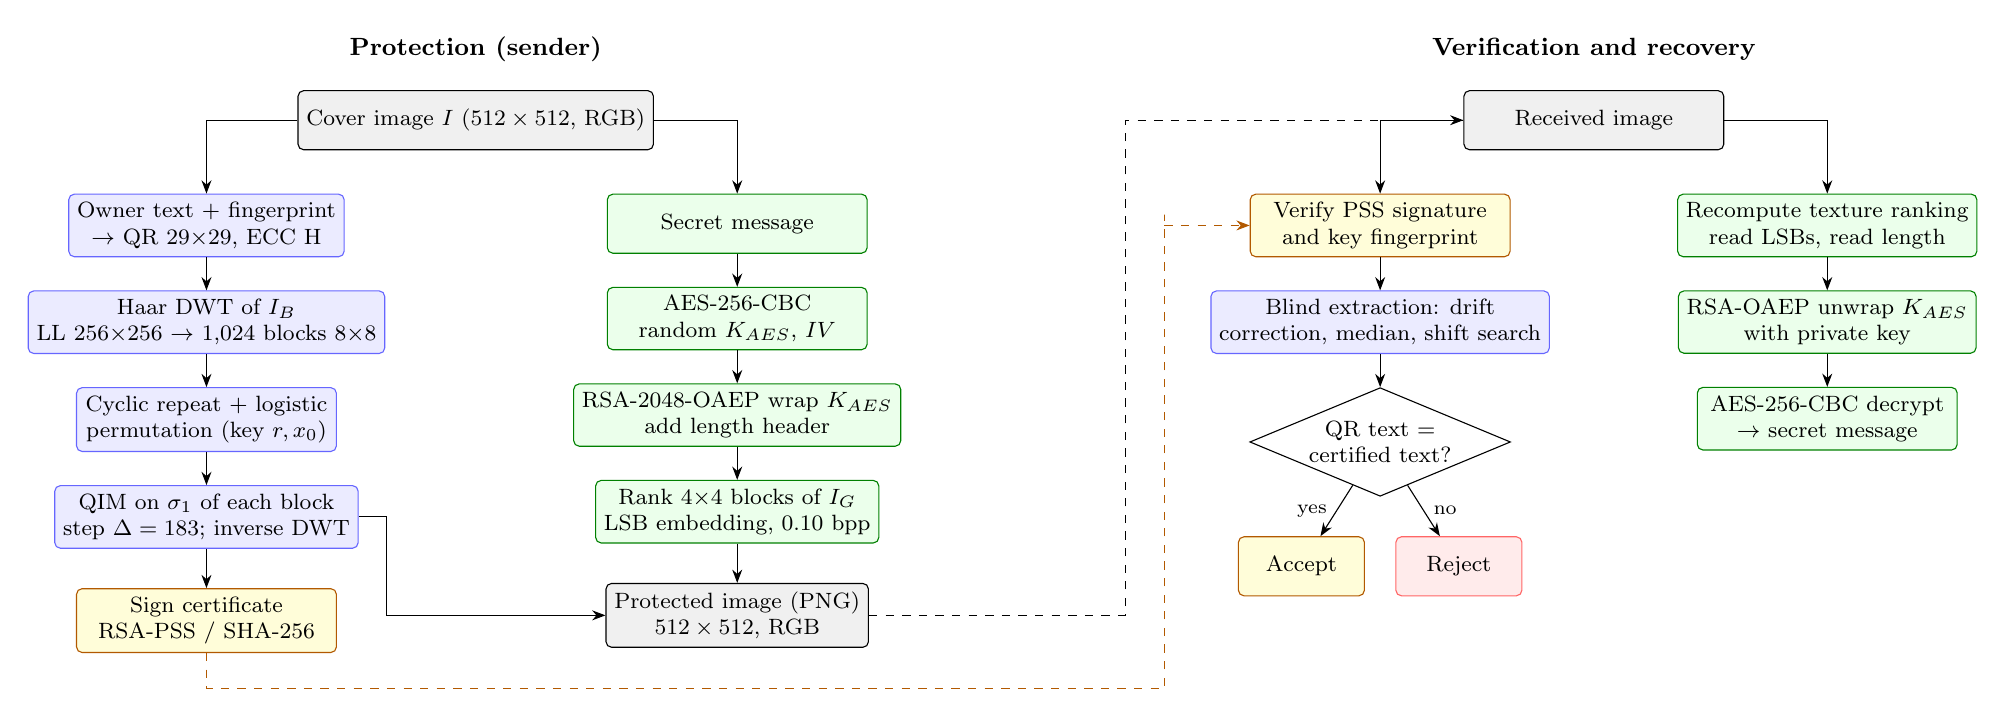
\begin{tikzpicture}[>=Stealth, node distance=0.42cm,
  st/.style={draw, rounded corners=2pt, align=center, font=\footnotesize, minimum width=3.3cm, minimum height=0.75cm, inner sep=3pt},
  wb/.style={st, fill=blue!8, draw=blue!60},
  gb/.style={st, fill=green!8, draw=green!50!black},
  cb/.style={st, fill=yellow!15, draw=orange!70!black},
  ib/.style={st, fill=gray!12},
  dec/.style={draw, diamond, aspect=2.4, align=center, font=\footnotesize, inner sep=1pt, fill=white}]
  \node[font=\bfseries\small] (S) at (0,0.9) {Protection (sender)};
  \node[ib] (c) at (0,0) {Cover image $I$ ($512\times512$, RGB)};
  \node[wb, below left=0.55cm and -0.6cm of c] (w1) {Owner text + fingerprint\\$\rightarrow$ QR $29{\times}29$, ECC H};
  \node[wb, below=of w1] (w2) {Haar DWT of $I_B$\\LL $256{\times}256$ $\rightarrow$ 1{,}024 blocks $8{\times}8$};
  \node[wb, below=of w2] (w3) {Cyclic repeat + logistic\\permutation (key $r, x_0$)};
  \node[wb, below=of w3] (w4) {QIM on $\sigma_1$ of each block\\step $\Delta=183$; inverse DWT};
  \node[gb, below right=0.55cm and -0.6cm of c] (g1) {Secret message};
  \node[gb, below=of g1] (g2) {AES-256-CBC\\random $K_{AES}$, $IV$};
  \node[gb, below=of g2] (g3) {RSA-2048-OAEP wrap $K_{AES}$\\add length header};
  \node[gb, below=of g3] (g4) {Rank $4{\times}4$ blocks of $I_G$\\LSB embedding, 0.10 bpp};
  \node[cb, below=0.5cm of w4] (cert) {Sign certificate\\RSA-PSS / SHA-256};
  \node[ib, below=0.5cm of g4] (out) {Protected image (PNG)\\$512\times512$, RGB};
  \draw[->] (c) -| (w1); \draw[->] (c) -| (g1);
  \draw[->] (w1)--(w2); \draw[->] (w2)--(w3); \draw[->] (w3)--(w4); \draw[->] (w4)--(cert);
  \draw[->] (g1)--(g2); \draw[->] (g2)--(g3); \draw[->] (g3)--(g4); \draw[->] (g4)--(out);
  \draw[->] (w4.east) -- ++(0.35,0) |- (out.west);
  \node[font=\bfseries\small] (R) at (14.2,0.9) {Verification and recovery};
  \node[ib] (r0) at (14.2,0) {Received image};
  \node[cb, below left=0.55cm and -0.6cm of r0] (v1) {Verify PSS signature\\and key fingerprint};
  \node[wb, below=of v1] (v2) {Blind extraction: drift\\correction, median, shift search};
  \node[dec, below=of v2] (v3) {QR text $=$\\certified text?};
  \node[cb, below=0.5cm of v3, xshift=-1.0cm, minimum width=1.6cm] (acc) {Accept};
  \node[st, below=0.5cm of v3, xshift=1.0cm, minimum width=1.6cm, fill=red!8, draw=red!60] (rej) {Reject};
  \node[gb, below right=0.55cm and -0.6cm of r0] (m1) {Recompute texture ranking\\read LSBs, read length};
  \node[gb, below=of m1] (m2) {RSA-OAEP unwrap $K_{AES}$\\with private key};
  \node[gb, below=of m2] (m3) {AES-256-CBC decrypt\\$\rightarrow$ secret message};
  \draw[->] (r0) -| (v1); \draw[->] (r0) -| (m1);
  \draw[->] (v1)--(v2); \draw[->] (v2)--(v3); \draw[->] (v3) -- node[left,font=\scriptsize]{yes} (acc); \draw[->] (v3) -- node[right,font=\scriptsize]{no} (rej);
  \draw[->] (m1)--(m2); \draw[->] (m2)--(m3);
  \draw[dashed, ->, orange!70!black] (cert.south) -- ++(0,-0.45) -| (8.75,-1.2) |- (v1.west);
  \coordinate (xo) at (8.25,0); \draw[dashed, ->] (out.east) -- (out.east -| xo) |- (r0.west);
\end{tikzpicture}}
\caption{\textbf{Methodology flowchart of the proposed system.} Left: protection, with the ownership layer (blue boxes), the confidential layer (green boxes) and certificate signing (yellow). Right: ownership verification (left column) and message recovery (right column). Dashed arrows: the protected image and the certificate travel to the receiver and verifier.}
\label{fig:flow}
\end{figure}

\subsection{Parameters, dataset and setup}

Tables~\ref{tab:params}--\ref{tab:setup} list the configuration of both schemes, the test images and attacks, and the experimental setup.

\begin{table}[!htbp]
\centering\small
\caption{Configuration of both schemes.}\label{tab:params}
\begin{tabularx}{\textwidth}{@{}lXX@{}}
\toprule
Item & Base scheme (A), reproduced from~\cite{sanivarapu2022} & Proposed \\
\midrule
Image size & $512\times512$ pixels, RGB, 8 bits per channel & same \\
Watermark & QR code of the owner text, $256\times256$ pixels & QR code of owner text $+$ 8-hex key fingerprint, $29\times29$ modules, error correction H \\
Scrambling & logistic map, $r=3.9999$, $x_0=0.12345$, on the $256\times256$ QR pixels & same map and key, on the 1{,}024 block positions \\
Embedding & blue channel, Haar DWT, SVD of the $256\times256$ LL band, singular values $S+\alpha S_W$, $\alpha=0.05$ & blue channel, Haar DWT, QIM on $\sigma_1$ of each $8\times8$ LL block ($16\times16$ pixels), $\Delta=183$ \\
Extraction & non-blind: cover image $+$ QR singular vectors & blind: image $+$ certificate; median and $\pm4$-pixel shift retries \\
Ownership proof & QR decodes & RSA-PSS/SHA-256 certificate verifies and matches the extracted QR \\
Hidden layer & none & AES-256-CBC, RSA-2048-OAEP key wrap, texture-ranked LSB in $4\times4$-pixel blocks of the green channel, 0.10 bpp \\
Key sizes & -- & RSA 2048 bits; AES 256 bits; IV 128 bits; SHA-256 \\
\bottomrule
\end{tabularx}
\end{table}

\begin{table}[!htbp]
\centering\small
\caption{Test images and attacks.}\label{tab:data}
\begin{tabularx}{\textwidth}{@{}lX@{}}
\toprule
Test images & Airplane, Boat, Einstein, Girl, House, House~2, Lake, Lena, Mandrill, Mona Lisa, Peppers, Tree: the 12 images of~\cite{sanivarapu2022}, each $512\times512$ pixels, RGB, 8 bits per channel. Figures use Peppers. \\
Steganalysis data & 494 patches of $128\times128$ pixels from the green channels of 11 of these images and 13 further standard images ($403\times610$ to $1000\times1280$ pixels) \\
Attacks & JPEG $Q=90,70,50$; Gaussian noise $v=0.001, 0.01$; salt \& pepper $d=0.01$; $3\times3$ mean blur; centre blanking (central $128\times128$ pixels set to zero, 6.25\% of the area); scaling to $256\times256$ and back to $512\times512$; rotation $2^\circ$; translation 2 pixels \\
Metrics & PSNR, SSIM; QR decodability, BER, NCC (as defined in~\cite{sanivarapu2022}); hidden-message recovery; RS estimate and SPAM detector error $P_E$~\cite{pevny2010spam}; entropy, $\chi^2$, adjacent-pixel correlation, NPCR/UACI; ownership-claim acceptance \\
\bottomrule
\end{tabularx}
\end{table}

\begin{table}[!htbp]
\centering\small
\caption{Experimental setup.}\label{tab:setup}
\begin{tabularx}{\textwidth}{@{}lX@{}}
\toprule
Hardware & Linux cloud container, Intel Xeon @ 2.10\,GHz, 2 vCPU, 7\,GB RAM; timings on one core % TODO: confirm this matches the machine of the reported run
\\
Language & Python 3 \\
Libraries & NumPy, OpenCV, PyWavelets (Haar DWT), scikit-image (SSIM), SciPy, scikit-learn (random forest), PyCryptodome (AES, RSA-OAEP, RSA-PSS), qrcode and pyzbar (QR generation and decoding), pandas, Matplotlib \\
Code & \url{https://github.com/nandikaagarwall/Hybrid-Image-Security} \\
\bottomrule
\end{tabularx}
\end{table}

% =====================================================================
\section{Results and Comparison}\label{sec:results}

All results are means over the 12 test images ($512\times512$ pixels each) unless stated otherwise. ``A'' denotes the base scheme as reproduced by us, using exactly the same images, attacks and metrics as the proposed scheme. Improvement percentages use $(\text{New}-\text{Old})/\text{Old}\times100$ for higher-is-better metrics and $(\text{Old}-\text{New})/\text{Old}\times100$ for lower-is-better metrics, so a positive value is always an improvement.

\FloatBarrier
\subsection{Imperceptibility and PSNR comparison}\label{sec:res-imp}

Table~\ref{tab:psnr} compares the PSNR of every watermarked image with the value reported by the base paper~\cite{sanivarapu2022} and with our reproduction of the base scheme. With both layers embedded, the proposed image has a mean PSNR of 40.19\,dB, against 40.12\,dB for the reproduced base scheme carrying the watermark alone ($+0.18\%$). The base paper reports 42.45\,dB, so the proposed scheme is 5.32\% lower than the reported value. Our reproduction keeps the published $\alpha=0.05$, which gives 40.12\,dB in our implementation, and the proposed QIM step was set to match it so that robustness is compared at equal quality. Peppers is the only image on which the proposed scheme exceeds the reported PSNR (40.42 vs 40.35\,dB). Per image, the proposed PSNR ranges from 39.85\,dB (Mona Lisa) to 40.74\,dB (House).
Table~\ref{tab:ssim} gives the SSIM values and the PSNR of the individual channels: the hidden message keeps the green channel at 61.14\,dB.

\begin{table}[!htbp]
\centering\small
\caption{PSNR (dB) of the watermarked images ($512\times512$ pixels) compared with the base paper. Reported: Table~2 of~\cite{sanivarapu2022}. A: base scheme reproduced by us. Proposed: watermark and 0.10\,bpp encrypted message both embedded. Improvement in percent, higher-is-better form.}\label{tab:psnr}
\begin{tabular}{@{}lccccc@{}}
\toprule
Image & Base paper (reported) & A (reproduced) & Proposed & Imp.\ vs reported (\%) & Imp.\ vs A (\%) \\
\midrule
Airplane & 41.81 & 40.15 & 40.04 & $-4.22$ & $-0.26$ \\
Boat & 42.65 & 40.13 & 40.03 & $-6.15$ & $-0.25$ \\
Einstein & 43.36 & 40.08 & 40.21 & $-7.25$ & $+0.33$ \\
Girl & 42.85 & 40.14 & 40.44 & $-5.63$ & $+0.75$ \\
House & 42.25 & 40.10 & 40.74 & $-3.57$ & $+1.60$ \\
House 2 & 41.74 & 40.11 & 40.20 & $-3.70$ & $+0.22$ \\
Lake & 41.68 & 40.07 & 40.05 & $-3.92$ & $-0.05$ \\
Lena & 42.22 & 40.14 & 40.13 & $-4.95$ & $-0.02$ \\
Mandrill & 43.12 & 40.11 & 40.00 & $-7.23$ & $-0.28$ \\
Mona Lisa & 43.81 & 40.10 & 39.85 & $-9.03$ & $-0.62$ \\
Peppers & 40.35 & 40.21 & 40.42 & $+0.17$ & $+0.51$ \\
Tree & 43.56 & 40.12 & 40.21 & $-7.69$ & $+0.23$ \\
\midrule
Mean & 42.45 & 40.12 & 40.19 & $-5.32$ & $+0.18$ \\
\bottomrule
\end{tabular}
\end{table}

\begin{table}[!htbp]
\centering\small
\caption{SSIM and per-channel PSNR of the watermarked images ($512\times512$ pixels). The red channel is not modified by either scheme.}\label{tab:ssim}
\resizebox{\textwidth}{!}{%
\begin{tabular}{@{}lcccc@{}}
\toprule
Image & A: SSIM & Proposed: SSIM & Proposed: blue PSNR (dB) & Proposed: green PSNR (dB) \\
\midrule
Airplane & 0.9934 & 0.9876 & 35.28 & 61.18 \\
Boat & 0.9963 & 0.9923 & 35.27 & 61.15 \\
Einstein & 0.9968 & 0.9917 & 35.45 & 61.17 \\
Girl & 0.9881 & 0.9877 & 35.68 & 61.13 \\
House & 0.9917 & 0.9901 & 35.98 & 61.14 \\
House 2 & 0.9958 & 0.9916 & 35.44 & 61.09 \\
Lake & 0.9971 & 0.9918 & 35.29 & 61.17 \\
Lena & 0.9953 & 0.9912 & 35.37 & 61.12 \\
Mandrill & 0.9984 & 0.9965 & 35.24 & 61.09 \\
Mona Lisa & 0.9865 & 0.9863 & 35.09 & 61.18 \\
Peppers & 0.9944 & 0.9898 & 35.66 & 61.13 \\
Tree & 0.9956 & 0.9915 & 35.45 & 61.12 \\
\midrule
Mean $\pm$ SD & $0.9941\pm0.0036$ & $0.9907\pm0.0027$ & $35.43\pm0.24$ & $61.14\pm0.03$ \\
\bottomrule
\end{tabular}}
\end{table}

Figure~\ref{fig:visual} shows the cover, the base-scheme image and the proposed image, with amplified difference images. Neither marked image shows visible artefacts. The difference images show where each layer acts. The base scheme's change follows the image's edges. The proposed watermark is spread evenly over $16\times16$-pixel blocks, each matching one $8\times8$ LL block. The hidden bits sit on edges and textured regions, where the texture ranking places them.

\begin{figure}[!htbp]
\centering
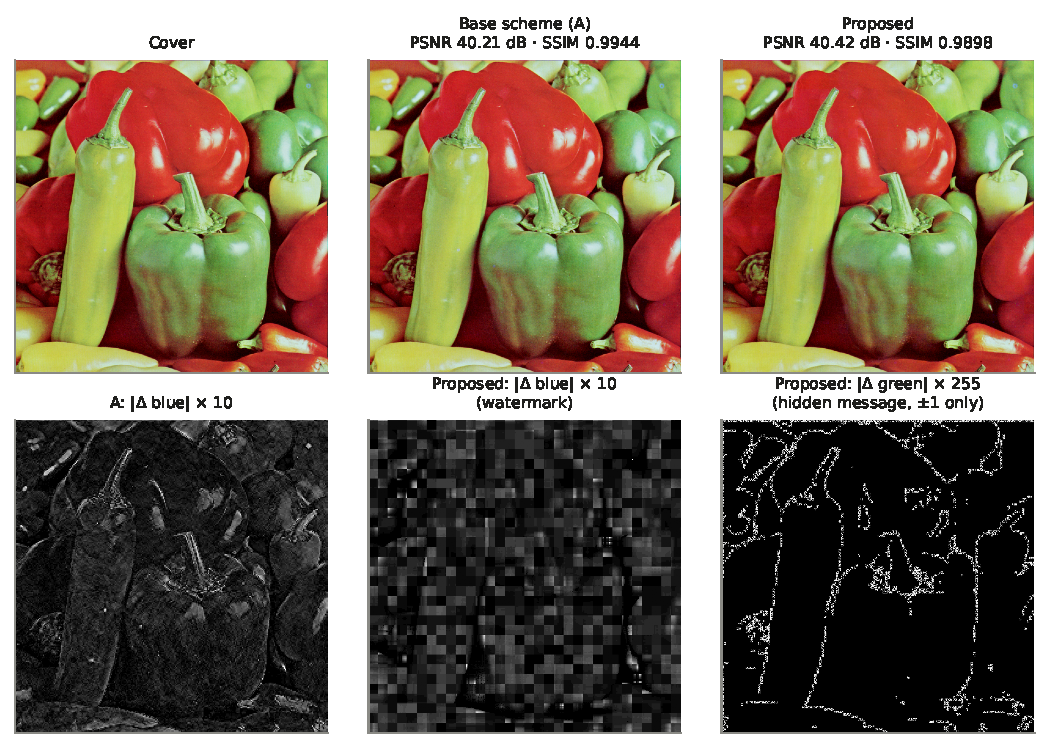
\includegraphics[width=0.92\textwidth]{F01_visual_quality}
\caption{\textbf{Visual quality} (Peppers, $512\times512$ pixels). Top: cover, base scheme (A) and proposed image with PSNR and SSIM. Bottom: absolute difference from the cover, amplified $\times10$ for the blue channel (watermark) and $\times255$ for the green channel (hidden message, where every change is $\pm1$).}
\label{fig:visual}
\end{figure}

Figure~\ref{fig:hist} examines the histograms of the embedded channels only, because the full RGB histogram cannot resolve changes of this size. On Peppers, the base scheme changes 89.2\% of the 262,144 blue pixels and raises their mean by 2.91 grey levels, so its histogram is visibly shifted (middle row). The proposed watermark changes 84.1\% of blue pixels with a mean change of $-0.15$, so its histogram stays centred on the cover's. The hidden message changes 5.03\% of green pixels, each by exactly $\pm1$ (bottom row, right).

\begin{figure}[!htbp]
\centering
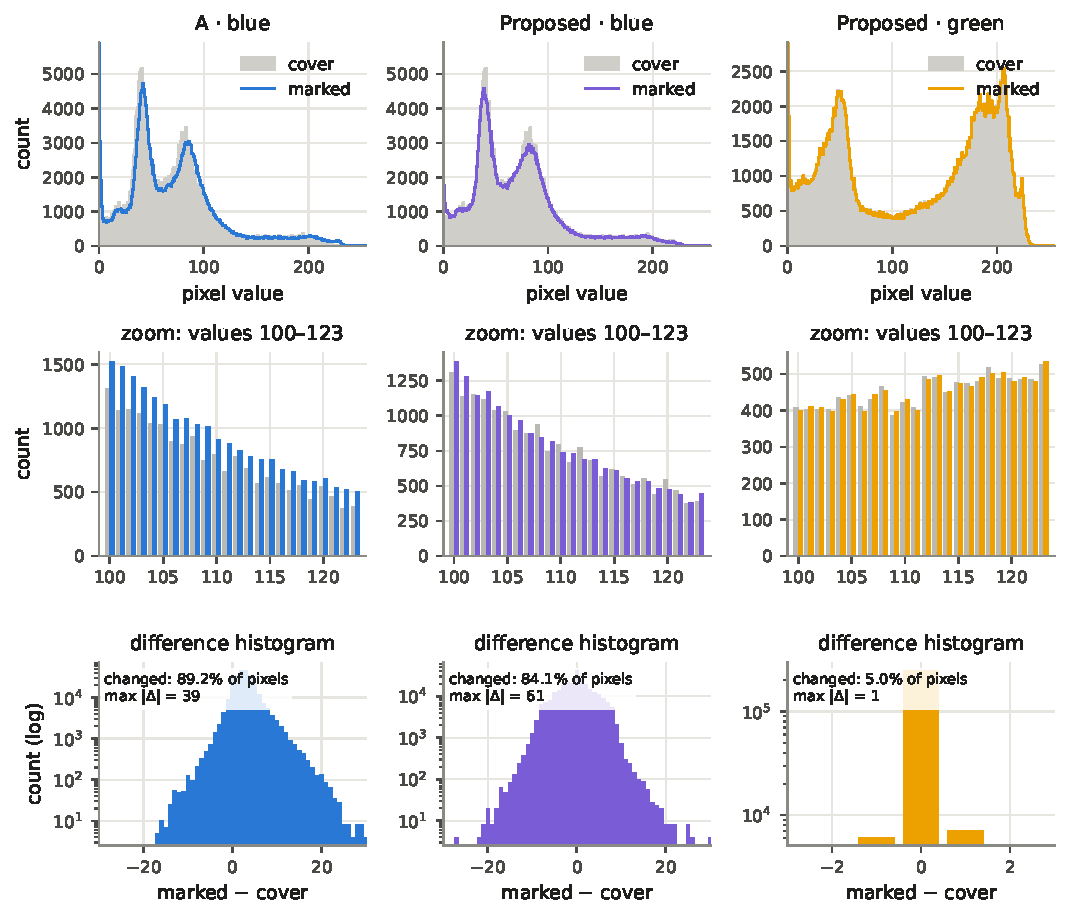
\includegraphics[width=0.92\textwidth]{F02_histograms}
\caption{\textbf{Histograms of the embedded channels} (Peppers, $512\times512$ pixels; cover in grey). Top: full range. Middle: zoom on values 100--123. Bottom: difference histogram, marked minus cover (log scale). Columns: base scheme blue channel, proposed blue channel (watermark), proposed green channel (hidden message).}
\label{fig:hist}
\end{figure}

\FloatBarrier
\subsection{Correlation analysis and encryption results}\label{sec:res-corr}

Figure~\ref{fig:corr} plots adjacent-pixel pairs of the embedded channels of the protected image in the horizontal, vertical and diagonal directions. For Peppers, the correlation coefficients of the blue channel change from $0.9665$, $0.9664$ and $0.9478$ to $0.9666$, $0.9665$ and $0.9477$, and those of the green channel ($0.9811$, $0.9818$ and $0.9687$) do not change at four decimals. Embedding therefore leaves the local structure of the image intact, as an imperceptible scheme should.

\begin{figure}[!htbp]
\centering
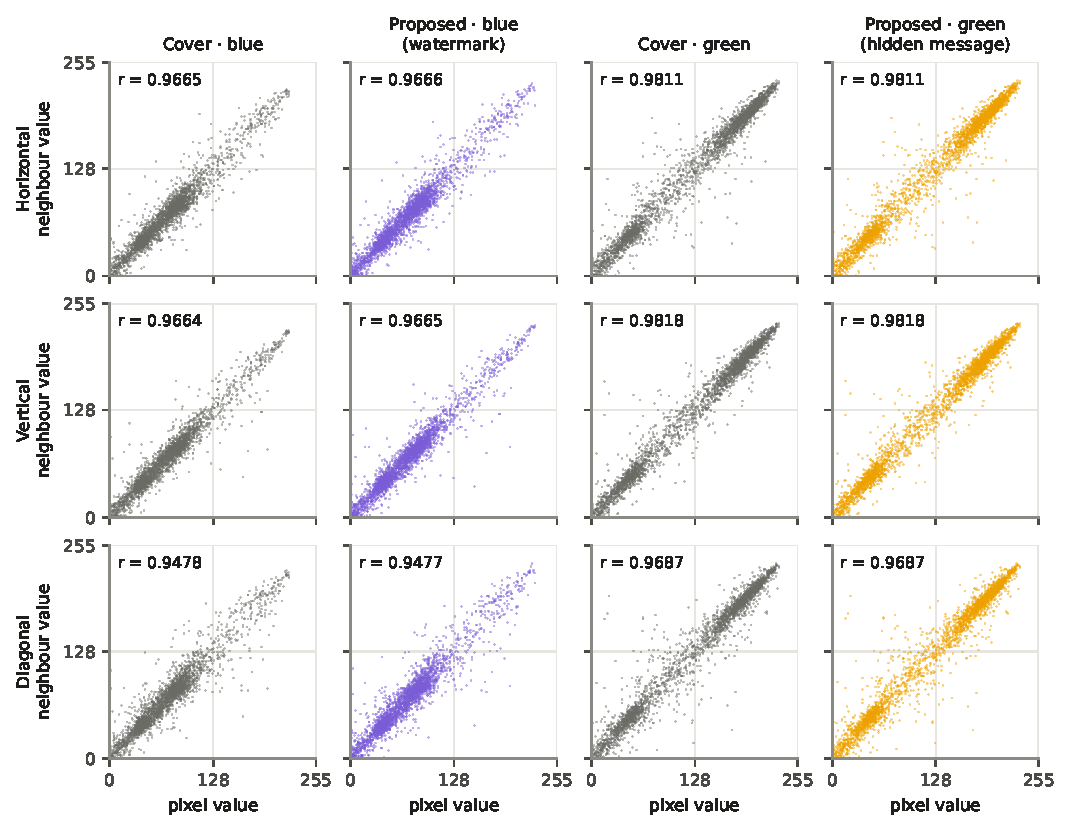
\includegraphics[width=0.85\textwidth]{F03_pixel_correlation}
\caption{\textbf{Adjacent-pixel correlation of the protected image} (Peppers, $512\times512$ pixels): cover vs proposed, blue and green channels, horizontal, vertical and diagonal neighbours. Each panel plots the same 3{,}000 random pixel pairs; $r$ is computed over all pairs.}
\label{fig:corr}
\end{figure}

The image itself is not encrypted: it carries the watermark and the hidden message. What is encrypted or scrambled is the watermark and the message, and Figure~\ref{fig:enc} shows what that does to them. The first two columns show the $256\times256$-pixel QR watermark before and after logistic-map scrambling. The plain QR code has strongly correlated neighbours ($r=0.884$, $0.866$ and $0.757$ horizontally, vertically and diagonally). After scrambling it looks like noise and the correlations drop to $-0.001$, $-0.003$ and $0.013$. Because the code is black and white, its scatter plots can only show four clusters; after scrambling the four clusters are equally populated, which is what zero correlation means for a binary image. The last two columns show 64\,KiB of message text and its AES-256-CBC ciphertext, each displayed as a $256\times256$ image with one byte per pixel. The plaintext occupies a narrow band of byte values (printable characters) in a repeating pattern. The ciphertext spreads uniformly over all 256 values, with correlations of $-0.013$, $0.004$ and $-0.011$. Table~\ref{tab:sec} in Section~\ref{sec:res-sec} gives the entropy and $\chi^2$ tests of the same ciphertext.

\begin{figure}[!htbp]
\centering
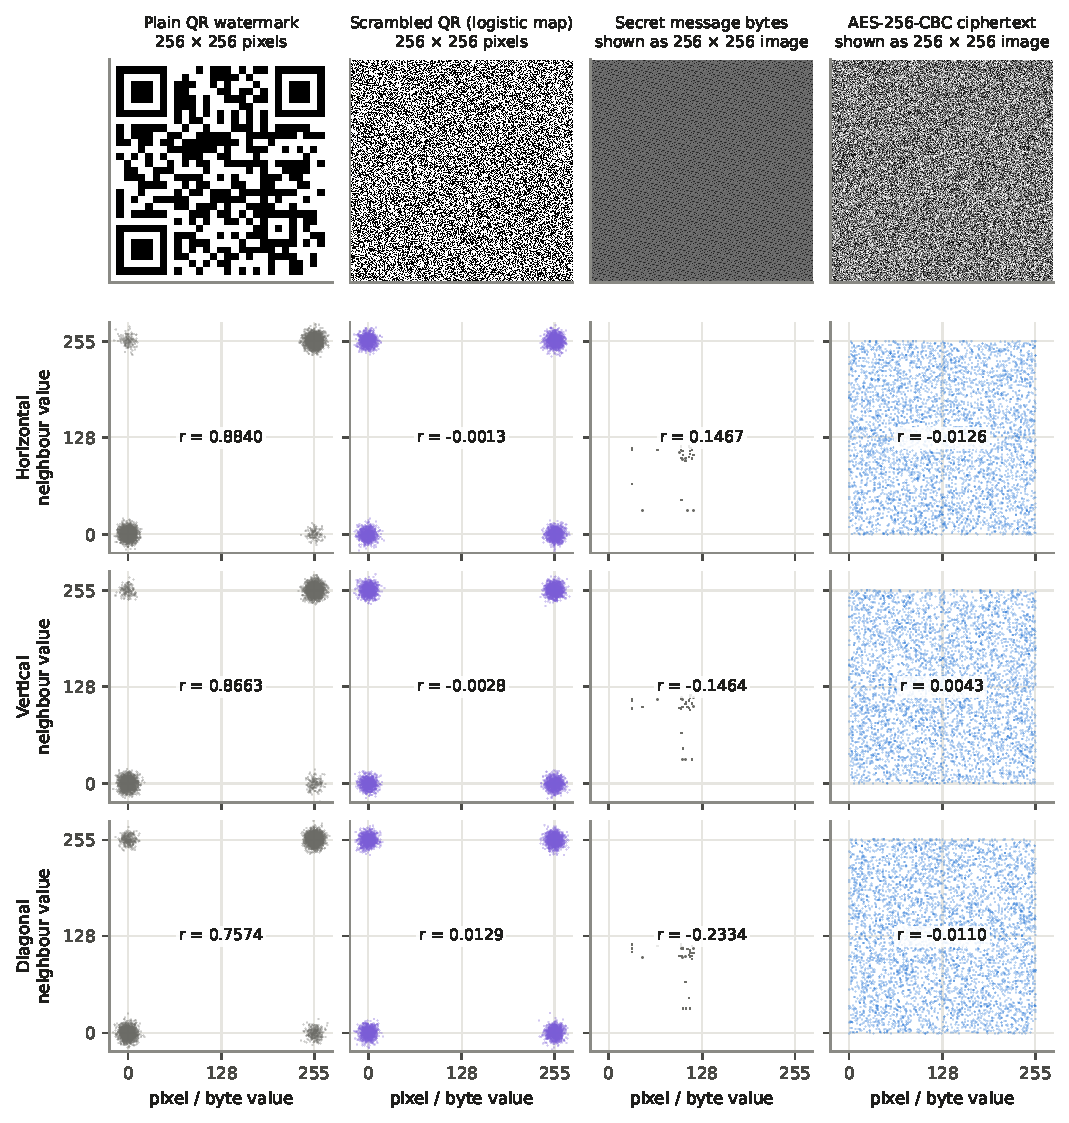
\includegraphics[width=0.92\textwidth]{F11_encryption_correlation}
\caption{\textbf{What encryption and scrambling do to the data.} Top row: the plain QR watermark and the scrambled QR ($256\times256$ pixels), and 64\,KiB of message text and its AES-256-CBC ciphertext, each shown as a $256\times256$ image with one byte per pixel. Rows 2--4: horizontal, vertical and diagonal neighbour pairs (5{,}000 random pairs per panel) with the correlation coefficient $r$. For the binary QR images the points are jittered slightly so that the four possible value pairs are visible.}
\label{fig:enc}
\end{figure}

\FloatBarrier
\subsection{Robustness}\label{sec:res-rob}

Table~\ref{tab:rob} reports how many of the 12 images still yield a decodable QR code after each attack, together with BER and NCC. Decodability is the primary measure. With the base scheme's extractor, an image that was never watermarked still scores NCC $=0.426$ (BER 54.1\%, 0/12 decodable), so NCC values in the 0.4--0.8 range do not indicate a recovered watermark.

\begin{table}[!htbp]
\centering\small
\caption{Robustness under attack (12 images of $512\times512$ pixels). BER for A is over the $256\times256$ QR pixels, for the proposed scheme over the $29\times29$ QR modules. Bold: more images decoded. Owner: ownership claim verified. Msg: hidden message recovered.}\label{tab:rob}
\resizebox{\textwidth}{!}{%
\begin{tabular}{@{}lccccccccc@{}}
\toprule
& & \multicolumn{3}{c}{Base scheme (A)} & \multicolumn{5}{c}{Proposed} \\
\cmidrule(lr){3-5}\cmidrule(lr){6-10}
Attack & Attacked PSNR (dB) & Decodes & BER\% & NCC & Decodes & BER\% & NCC & Owner & Msg \\
\midrule
No attack & -- & 12/12 & 0.0 & 1.000 & 12/12 & 0.0 & 1.000 & 12/12 & 12/12 \\
JPEG $Q=90$ & 33.62 & 12/12 & 5.5 & 0.947 & 12/12 & 0.0 & 1.000 & 12/12 & 0/12 \\
JPEG $Q=70$ & 31.72 & 8/12 & 14.4 & 0.901 & \textbf{12/12} & 0.2 & 0.997 & 12/12 & 0/12 \\
JPEG $Q=50$ & 30.68 & 8/12 & 16.1 & 0.886 & \textbf{12/12} & 0.9 & 0.991 & 12/12 & 0/12 \\
Gaussian $v=0.001$ & 29.62 & 12/12 & 0.0 & 0.998 & 12/12 & 0.0 & 1.000 & 12/12 & 0/12 \\
Gaussian $v=0.01$ & 20.20 & \textbf{12/12} & 1.4 & 0.989 & 0/12 & 8.7 & 0.908 & 0/12 & 0/12 \\
Salt \& pepper $d=0.01$ & 20.35 & \textbf{12/12} & 3.0 & 0.979 & 9/12 & 7.9 & 0.918 & 9/12 & 0/12 \\
Mean blur $3\times3$ & 30.62 & 1/12 & 52.4 & 0.608 & \textbf{11/12} & 0.6 & 0.993 & 11/12 & 0/12 \\
Centre blanking ($128\times128$) & 16.99 & 0/12 & 42.5 & 0.559 & \textbf{12/12} & 2.2 & 0.977 & 12/12 & 4/12 \\
Scaling $512\to256\to512$ & 30.24 & 2/12 & 53.7 & 0.604 & \textbf{11/12} & 0.3 & 0.996 & 11/12 & 0/12 \\
Rotation $2^\circ$ & 17.43 & 0/12 & 28.9 & 0.782 & 0/12 & 41.4 & 0.568 & 0/12 & 0/12 \\
Translation 2 pixels & 19.60 & 12/12 & 0.1 & 0.999 & 12/12 & 1.3 & 0.987 & 12/12 & 0/12 \\
\midrule
Total (11 attacks) & & 79/132 & & & \textbf{103/132} & & & 103/132 & 4/132 \\
\bottomrule
\end{tabular}}
\end{table}

The proposed watermark decodes on more images than the base scheme under five attacks and ties under four. It decodes on fewer images under heavy Gaussian noise and salt \& pepper. Neither scheme survives a $2^\circ$ rotation, which moves pixels near the corners of a $512\times512$ image by about 13 pixels, beyond the decoder's 4-pixel search. Wherever the QR code decodes, the ownership claim also verifies. The hidden message survives only the clean channel and, on 4 images, centre blanking, where its bits lie outside the blanked $128\times128$ square. This is expected for spatial-domain LSB embedding, so the protected image must be shared losslessly.

Table~\ref{tab:psnr-att} compares the PSNR of the attacked images with the values reported by the base paper. Here PSNR measures how strongly each attack degrades the image, not the quality of the watermark, so it is not scored as an improvement. Our attacked images have markedly lower PSNR: after Gaussian noise of variance 0.01, for example, 20.20\,dB against the reported 38.80\,dB. This indicates that the base paper's attacks were milder than ours or that its PSNR was computed against a different reference. The robustness results in Table~\ref{tab:rob} were therefore obtained under harder conditions than those reported in~\cite{sanivarapu2022}.

\begin{table}[!htbp]
\centering\small
\caption{PSNR (dB) of the attacked watermarked images ($512\times512$ pixels), mean over 12 images: values reported in Tables~3--4 of~\cite{sanivarapu2022} with the base paper's attack settings, and our values for the proposed scheme with the settings of Table~\ref{tab:data}. Lower values mean a stronger attack.}\label{tab:psnr-att}
\begin{tabular}{@{}llcc@{}}
\toprule
Attack (ours) & Base paper setting & Base paper (reported) & Proposed (ours) \\
\midrule
JPEG $Q=90$ & $Q=90$ & 37.23 & 33.62 \\
Gaussian $v=0.01$ & variance 0.01 & 38.80 & 20.20 \\
Salt \& pepper $d=0.01$ & density 0.5 (as stated) & 35.75 & 20.35 \\
Mean blur $3\times3$ & mean filter $3\times3$ & 33.17 & 30.62 \\
Centre blanking ($128\times128$) & cropping, size not stated & 29.16 & 16.99 \\
Scaling $512\to256\to512$ & down-sampled twice & 38.78 & 30.24 \\
Rotation $2^\circ$ & angle not stated & 28.64 & 17.43 \\
Translation 2 pixels & 2 pixels in $x$ and $y$ & 36.25 & 19.60 \\
\bottomrule
\end{tabular}
\end{table}

Figure~\ref{fig:grid} shows the QR codes extracted by both schemes from the attacked Peppers image. Under blur, centre blanking and rescaling, the base scheme returns noise while the proposed scheme returns a readable code. Under heavy Gaussian noise the proposed code has a module BER of 10.7\% and does not decode.

\begin{figure}[!htbp]
\centering
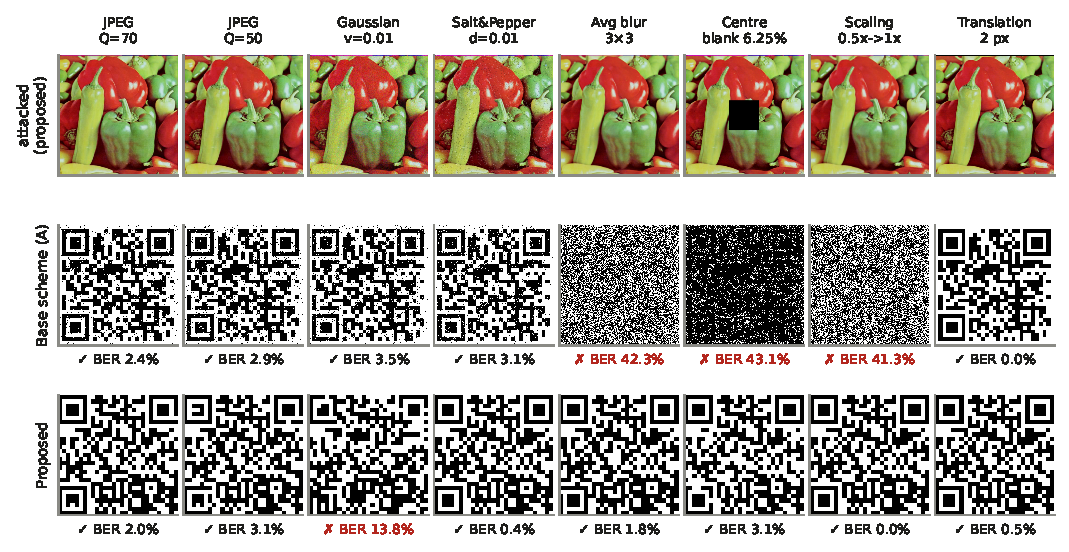
\includegraphics[width=\textwidth]{F04_attack_grid}
\caption{\textbf{Attacked images and extracted watermarks} (Peppers, $512\times512$ pixels). Top: attacked proposed images. Middle: QR codes ($256\times256$ pixels) extracted by the base scheme. Bottom: QR codes ($29\times29$ modules) extracted by the proposed scheme. Below each: BER and whether the code decodes (\checkmark/$\times$).}
\label{fig:grid}
\end{figure}

Figure~\ref{fig:strength} sweeps the attack strength. Under JPEG the proposed watermark decodes on all 12 images down to $Q=50$ and on 8 at $Q=40$, while the base scheme already loses images at $Q=80$ (10/12). Under Gaussian noise the proposed watermark holds 12/12 up to variance 0.002 and 11/12 at 0.005, then fails; the base scheme holds 12/12 throughout. Under salt \& pepper the proposed watermark stays at 9--10 of 12 up to density 0.05.

\begin{figure}[!htbp]
\centering
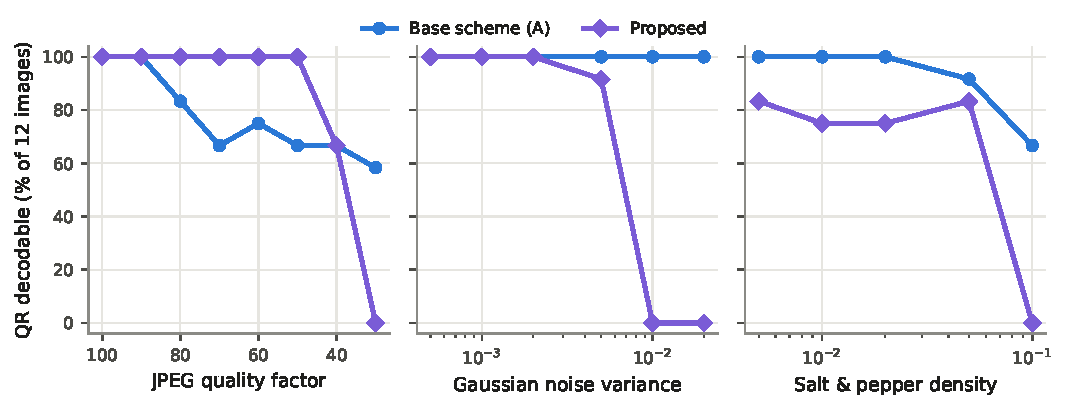
\includegraphics[width=\textwidth]{F05_robustness_vs_strength}
\caption{\textbf{Robustness against attack strength.} Share of the 12 test images ($512\times512$ pixels) whose QR code decodes as the JPEG quality falls and as the Gaussian noise variance and salt \& pepper density rise.}
\label{fig:strength}
\end{figure}

\FloatBarrier
\subsection{Imperceptibility--robustness trade-off}\label{sec:res-trade}

The noise weakness follows from the chosen operating point. Figure~\ref{fig:trade} varies the embedding strength of both schemes. At a QIM step of 240 (PSNR 37.73\,dB), the proposed watermark decodes on 12/12 images under JPEG-70, Gaussian noise of variance 0.01 and salt \& pepper alike. The base scheme needs $\alpha=0.10$ (PSNR 33.81\,dB) to reach 12/12 under JPEG-70, and has only 8/12 at its published $\alpha=0.05$.

\begin{figure}[!htbp]
\centering
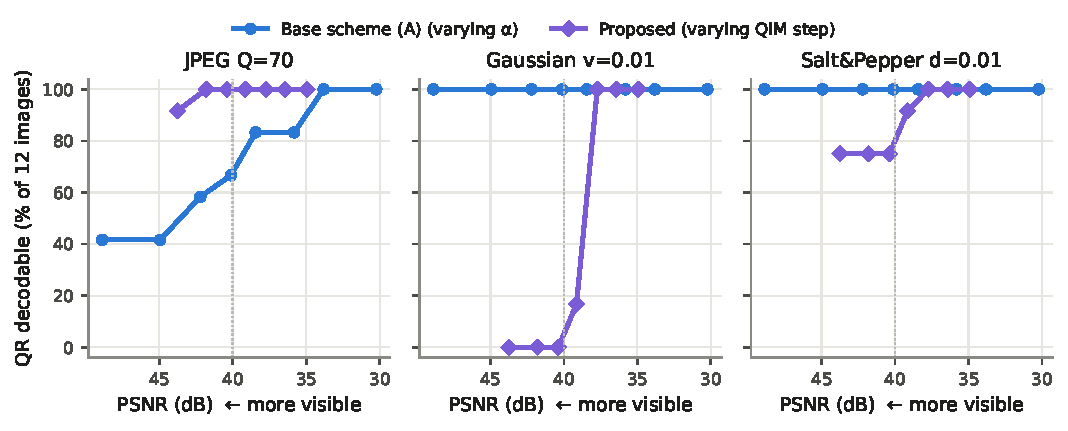
\includegraphics[width=\textwidth]{F06_tradeoff}
\caption{\textbf{Imperceptibility--robustness trade-off.} Share of the 12 test images whose QR code decodes against the PSNR of the marked image, varying $\alpha$ for the base scheme and the QIM step for the proposed scheme. Dotted line: the 40\,dB operating point of Tables~\ref{tab:psnr} and~\ref{tab:rob}.}
\label{fig:trade}
\end{figure}

\FloatBarrier
\subsection{Hidden layer: capacity and detectability}\label{sec:res-hidden}

Table~\ref{tab:hidden} and Figure~\ref{fig:hidden} evaluate the green-channel layer from 0.05 to 0.40 bits per pixel (13,107 to 104,857 bits in a $512\times512$ channel). The real 340-byte payload is padded with random bits to each rate. The message is recovered in all 55 clean runs. Texture-ranked and random placement give the same PSNR, since both change about half of the used pixels by one level, but they differ in detectability. RS analysis, which recovers the payload of random LSB embedding almost exactly (0.404 for a true 0.40\,bpp), estimates only 0.199 for texture-ranked embedding. % CITATION NEEDED: RS steganalysis (Fridrich, Goljan and Du, 2001)
The learned SPAM detector~\cite{pevny2010spam} also errs more often on texture-ranked embedding ($P_E=0.397$ vs 0.348 at 0.10\,bpp). This result is preliminary: it uses 494 patches of $128\times128$ pixels, and a full evaluation on BOSSbase~\cite{bas2011boss} remains to be done.

\begin{table}[!htbp]
\centering\small
\caption{Hidden-layer capacity and detectability in the green channel ($512\times512$ pixels). RS estimate: embedding rate inferred by RS analysis (0.022 on unmodified covers; closer to the true rate means easier to detect). $P_E$: detection error of SPAM features with a random forest (0.5 = undetectable). PSNR and recovery over 11 images; RS over 12.}\label{tab:hidden}
\begin{tabular}{@{}cccccccc@{}}
\toprule
& & & & \multicolumn{2}{c}{RS estimate} & \multicolumn{2}{c}{$P_E$} \\
\cmidrule(lr){5-6}\cmidrule(lr){7-8}
bpp & Bits & Green PSNR (dB) & Recovered & Ours & Random LSB & Ours & Random LSB \\
\midrule
0.05 & 13{,}107 & 64.15 & 11/11 & \textbf{0.034} & 0.061 & -- & -- \\
0.10 & 26{,}214 & 61.13 & 11/11 & \textbf{0.049} & 0.112 & \textbf{0.397} & 0.348 \\
0.20 & 52{,}428 & 58.13 & 11/11 & \textbf{0.083} & 0.209 & \textbf{0.374} & 0.336 \\
0.30 & 78{,}643 & 56.38 & 11/11 & \textbf{0.130} & 0.305 & -- & -- \\
0.40 & 104{,}857 & 55.12 & 11/11 & \textbf{0.199} & 0.404 & \textbf{0.338} & 0.299 \\
\bottomrule
\end{tabular}
\end{table}

\begin{figure}[!htbp]
\centering
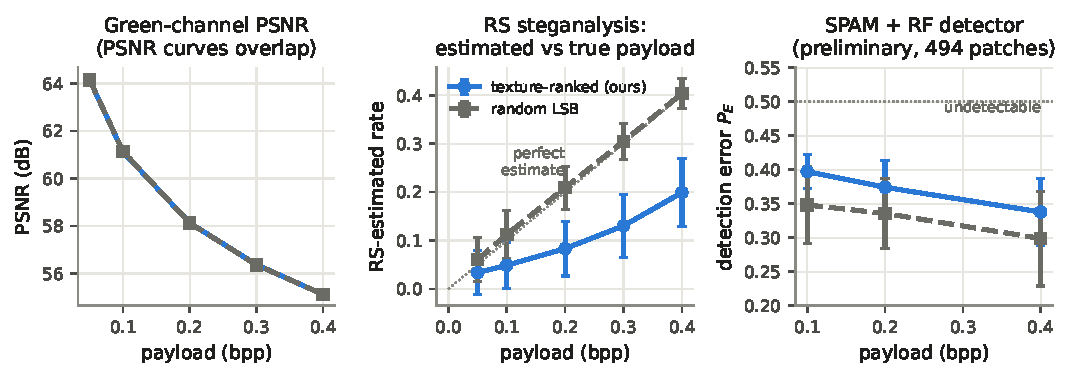
\includegraphics[width=\textwidth]{F07_hidden_layer}
\caption{\textbf{Hidden layer} ($512\times512$-pixel green channels). Left: green-channel PSNR against payload. Centre: RS-estimated against true payload (dotted: perfect estimate). Right: SPAM detector error (dotted: undetectable).}
\label{fig:hidden}
\end{figure}

\FloatBarrier
\subsection{Security of the cryptographic components}\label{sec:res-sec}

Table~\ref{tab:sec} summarises the randomness and key-sensitivity tests. The AES-256-CBC ciphertext of Figure~\ref{fig:enc} has an entropy of 7.9975 bits per byte and a byte-histogram $\chi^2$ of 227.9, below the 5\% critical value of 293.25, so it is statistically indistinguishable from uniform. A one-bit change in the first plaintext byte changes 99.60\% of ciphertext bytes (UACI 33.35\%), and a one-bit change in the key changes 99.61\% of the decrypted bytes. These figures are measured on 64\,KiB of ciphertext because the 64-byte message alone is too short for byte statistics. A change in the \emph{last} plaintext byte changes only 0.02\% of the ciphertext, since CBC propagates changes forward only.

For the watermark key, changing $x_0$ by $10^{-10}$ yields a module BER of 0.474 and no QR code (Figure~\ref{fig:scramble}), and none of 300 random $(r,x_0)$ keys yields any decodable QR code from a marked image, even with the full decoder including the shift search. Logistic-map scrambling removes the correlation of the QR code (Figure~\ref{fig:enc}). Because it is a permutation, however, it leaves the histogram and entropy unchanged and is known to be breakable by chosen-plaintext attacks~\cite{TODO}. % CITATION NEEDED: cryptanalysis of permutation-only ciphers (e.g., Jolfaei, Wu and Muthukkumarasamy, IEEE TIFS 2016)
In this scheme it serves to spread burst errors and to key the bit positions; confidentiality rests on AES and RSA.

\begin{table}[!htbp]
\centering\small
\caption{Security tests of the encryption and scrambling components.}\label{tab:sec}
\begin{tabularx}{\textwidth}{@{}p{3.1cm}X>{\raggedright\arraybackslash}p{4.6cm}>{\raggedright\arraybackslash}p{2.2cm}@{}}
\toprule
Component & Test & Value & Ideal \\
\midrule
AES-256-CBC & Entropy (bits/byte) & 7.9975 & 8 \\
AES-256-CBC & $\chi^2$ of byte histogram & 227.9 & $<293.25$ \\
AES-256-CBC & Adjacent-byte correlation H / V / D & $-0.013$ / $0.004$ / $-0.011$ & 0 \\
AES-256-CBC & NPCR / UACI, 1-bit change in the first byte & 99.60\% / 33.35\% & 99.61\% / 33.46\% \\
AES-256-CBC & Bytes changed by a 1-bit change in the key & 99.61\% & $\approx$99.6\% \\
Logistic map (QR, $256\times256$ pixels) & Correlation H / V / D, plain $\rightarrow$ scrambled & $0.884\rightarrow-0.001$ / $0.866\rightarrow-0.003$ / $0.757\rightarrow0.013$ & $\rightarrow0$ \\
Logistic key, base scheme & Watermark BER with $x_0+10^{-10}$ & 0.497 & 0.5 \\
Logistic key, proposed & Module BER with $x_0+10^{-10}$ & 0.474 (no QR) & 0.5 \\
Proposed watermark key & Random keys giving any decodable QR & 0 of 300 & 0 \\
\bottomrule
\end{tabularx}
\end{table}

\begin{figure}[!htbp]
\centering
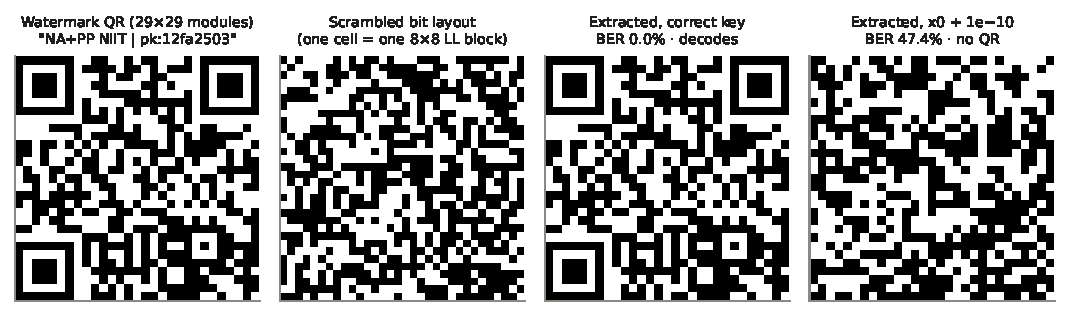
\includegraphics[width=\textwidth]{F08_scrambling_key_sensitivity}
\caption{\textbf{Key sensitivity of the proposed watermark.} From left: the QR code ($29\times29$ modules: owner text and public-key fingerprint), its scrambled layout over the 1{,}024 LL blocks ($32\times32$ grid), the QR code extracted from a marked $512\times512$ image with the correct key, and with $x_0$ changed by $10^{-10}$.}
\label{fig:scramble}
\end{figure}

\FloatBarrier
\subsection{Ownership verification}\label{sec:res-own}

Table~\ref{tab:own} reports the ownership tests, and Figure~\ref{fig:own} shows the central one. Against the base scheme, an attacker generates a QR code of their own identity, scrambles it with the same map, and presents its singular vectors as their key. Applied to the owner's image, these vectors extract the attacker's QR code, which decodes on 12/12 images. Against the proposed scheme, the attacker presents a correctly signed certificate for their own key and parameters. Blind extraction with those parameters yields no QR code on any image, so the claim is rejected (0/12). Editing the owner's certificate breaks its signature, and re-signing the owner's parameters with the attacker's key fails because the QR text in the image carries the owner's fingerprint. Neither scheme accepts a claim on an image that was never watermarked.

\begin{table}[!htbp]
\centering\small
\caption{Ownership-verification tests (12 images of $512\times512$ pixels each).}\label{tab:own}
\resizebox{\textwidth}{!}{%
\begin{tabular}{@{}lccc@{}}
\toprule
Claim & A: accepted & Proposed: accepted & Correct \\
\midrule
Real owner claims the marked image & 12/12 & 12/12 & accept \\
Attacker presents own keys (false-ownership attack) & 12/12 & \textbf{0/12} & reject \\
Owner's certificate with the owner field edited & no certificate & 0/12 & reject \\
Owner's parameters re-signed with the attacker's key & no certificate & 0/12 & reject \\
Owner's claim on an unmarked image & 0/12 & 0/12 & reject \\
Owner's claim on an unmarked image after JPEG-90 & -- & 0/12 & reject \\
Attacker re-watermarks the image with their own mark & -- & attacker 12/12, owner 0/12 & see text \\
\bottomrule
\end{tabular}}
\end{table}

\begin{figure}[!htbp]
\centering
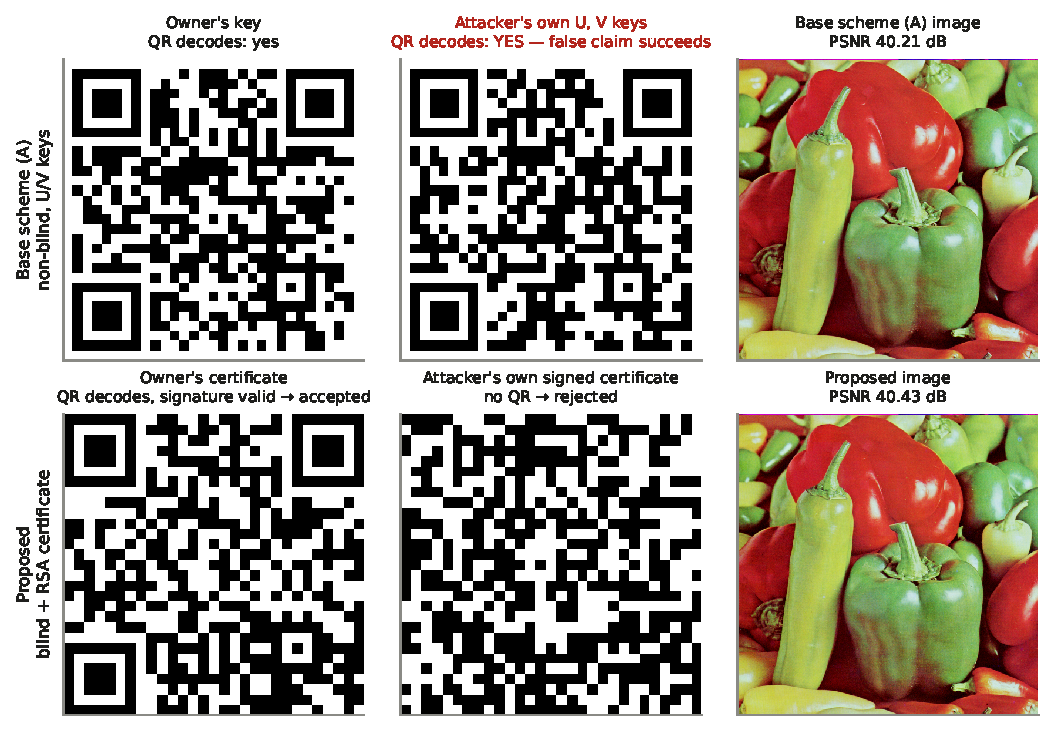
\includegraphics[width=0.88\textwidth]{F09_ownership_attack}
\caption{\textbf{False-ownership attack} (Peppers, $512\times512$ pixels). Top: base scheme; the attacker's own singular vectors extract the attacker's QR code from the owner's image. Bottom: proposed scheme; the owner's certificate verifies, and the attacker's own signed certificate yields no QR code.}
\label{fig:own}
\end{figure}

The last row of Table~\ref{tab:own} is a limitation. An attacker who re-embeds their own proposed-scheme watermark over the owner's (PSNR about 40\,dB against the cover) replaces it, because both marks use the same blocks. No blind scheme prevents this on its own. The standard remedy is a trusted timestamp on the signed certificate, so that the first registration wins~\cite{TODO}. % CITATION NEEDED: trusted time-stamping (RFC 3161)

\FloatBarrier
\subsection{Comparison with the base paper and similar work}\label{sec:res-cmp}

Table~\ref{tab:cmp} compares the proposed scheme with the values reported by the base paper~\cite{sanivarapu2022} and with our reproduction of it, and gives the improvement percentage for each metric. Two cautions apply to the reported values. First, Table~\ref{tab:psnr-att} shows that the base paper's attacks were milder than ours, and it does not state its cropping or rotation sizes. Second, our reproduction of its scheme reaches much lower NCC than reported under blur (0.608 vs 0.991), rescaling (0.604 vs 0.996) and rotation (0.782 vs 0.990). We therefore treat the comparison with the reproduced scheme, run under identical conditions, as the primary one. Figure~\ref{fig:cmp} shows the NCC comparison and the decodability counts.

\begin{table}[!htbp]
\centering\small
\caption{Comparison and improvement percentage. Reported: values published in~\cite{sanivarapu2022} (means over its 12 images). A: the same scheme reproduced under our conditions. Form H: $(\text{New}-\text{Old})/\text{Old}\times100$; form L: $(\text{Old}-\text{New})/\text{Old}\times100$.}\label{tab:cmp}
\resizebox{\textwidth}{!}{%
\begin{tabular}{@{}lcccccc@{}}
\toprule
& & \multicolumn{2}{c}{vs base paper (reported)} & \multicolumn{2}{c}{vs base scheme (A, reproduced)} & \\
\cmidrule(lr){3-4}\cmidrule(lr){5-6}
Metric & Proposed & Old & Imp.\,\% & Old & Imp.\,\% & Form \\
\midrule
PSNR (dB) & 40.19 & 42.45 & $-5.32$ & 40.12 & $+0.18$ & H \\
SSIM & 0.9907 & -- & -- & 0.9941 & $-0.35$ & H \\
NCC, JPEG $Q=90$ & 0.9998 & 0.9933 & $+0.65$ & 0.9467 & $+5.61$ & H \\
NCC, Gaussian $v=0.01$ & 0.9081 & 0.9900 & $-8.27$ & 0.9892 & $-8.20$ & H \\
NCC, salt \& pepper & 0.9178 & 0.9841 & $-6.74$ & 0.9791 & $-6.26$ & H \\
NCC, mean blur $3\times3$ & 0.9932 & 0.9909 & $+0.23$ & 0.6081 & $+63.31$ & H \\
NCC, scaling & 0.9964 & 0.9957 & $+0.06$ & 0.6037 & $+65.05$ & H \\
NCC, rotation $2^\circ$ & 0.5679 & 0.9898 & $-42.62$ & 0.7822 & $-27.40$ & H \\
NCC, translation 2 pixels & 0.9865 & 0.9781 & $+0.87$ & 0.9988 & $-1.23$ & H \\
Decodable cases (of 132) & 103 & -- & -- & 79 & $+30.38$ & H \\
False-ownership acceptance & 0\% & not evaluated & -- & 100\% & $+100.00$ & L \\
Verifier key material (bytes) & 758 & -- & -- & 1{,}835{,}008 & $+99.96$ & L \\
Embedding time (s) & 0.291 & -- & -- & 0.063 & $-360.9$ & L \\
Extraction time (s) & 1.544 & -- & -- & 0.125 & $-1135.7$ & L \\
\midrule
\multicolumn{7}{@{}l}{\todo{Similar paper 2: values and improvement \% to be added}} \\
\multicolumn{7}{@{}l}{\todo{Similar paper 3: values and improvement \% to be added}} \\
\bottomrule
\end{tabular}}
\end{table}
% Values: paper/out/robustness.csv (A), final_robustness_P.csv and final_imperceptibility_P.csv (proposed),
% paper/base_paper.py (reported). Key material for A = the QR singular vectors as float64 (2 x 256 x 256 x 8 B)
% + the cover image (512 x 512 x 3 B); for the proposed scheme = the certificate JSON incl. signature.

\begin{figure}[!htbp]
\centering
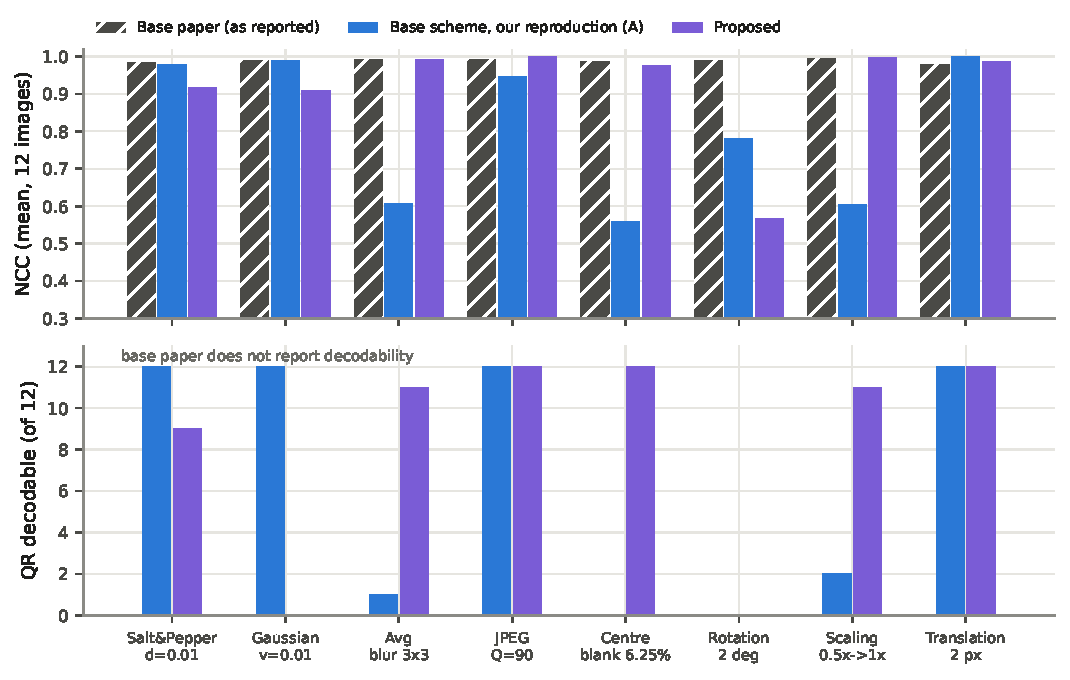
\includegraphics[width=0.92\textwidth]{F10_comparison_base_paper}
\caption{\textbf{Comparison with the base paper.} Top: mean NCC as reported by the base paper, for our reproduction of it, and for the proposed scheme (12 images, $512\times512$ pixels). Bottom: images (of 12) whose QR code still decodes, which the base paper does not report.}
\label{fig:cmp}
\end{figure}

\paragraph{Why the proposed scheme performs better.} Three design choices explain the gains. (i) Each module is read from the \emph{position} of $\sigma_1$ within a quantisation cell, not from a difference with the cover. A module flips only if an attack moves $\sigma_1$ by more than $\Delta/4\approx46$ from its cell centre. The low module BERs after blur (0.6\%), rescaling (0.3\%) and JPEG $Q=50$ (0.9\%) show that these low-pass operations rarely do so, whereas the base scheme divides every change in the singular values by $\alpha=0.05$, amplifying it twentyfold. (ii) Scrambling and cyclic repetition spread each module over the image, and the QR code's error correction absorbs the remaining module errors. This is why centre blanking, which destroys 64 of the 1,024 blocks, still decodes on 12/12 images. (iii) Blind extraction removes the claimant's influence on the result, which is what defeats the false-ownership attack. It also removes the need to store the cover image and singular vectors.

\paragraph{Where it does not.} The base scheme's extractor uses the QR code's own singular vectors, which carry most of the code's structure. This gives it strong immunity to additive noise, at the price of the ownership flaw. The blind scheme lacks this side information, so heavy Gaussian noise (attacked PSNR 20.2\,dB) and salt \& pepper reduce its decodability at 40\,dB; a lower PSNR operating point restores it (Section~\ref{sec:res-trade}). The proposed scheme is also slower: about 0.29\,s to embed versus 0.06\,s, and 1.54\,s to extract versus 0.13\,s. Extraction includes the hidden message, the certificate check and, after geometric attacks, the shift search. Neither scheme handles rotation.

% =====================================================================
\section{Conclusion}\label{sec:conclusion}

We reproduced the DWT--SVD QR watermarking scheme of~\cite{sanivarapu2022} on its 12 test images of $512\times512$ pixels and showed that it accepts false ownership claims on all of them. We then proposed a hybrid scheme with two layers in two colour channels. The blue channel carries a blind QIM watermark on block singular values, bound to the owner by an RSA-PSS-signed certificate. The green channel carries an AES-256/RSA-2048 encrypted message hidden by texture-ranked LSB. At the same image quality as the base scheme (40.19 vs 40.12\,dB), the proposed scheme rejects every false-ownership, forged-certificate and re-signed-certificate claim. Its watermark decodes on 103 of 132 attack--image cases against 79, and it delivers a confidential message that classical steganalysis underestimates by half.

Expressed as ``how many times better'' (New/Old for higher-is-better and Old/New for lower-is-better metrics), against the base scheme reproduced under identical conditions:
\begin{itemize}
  \item decodable attack cases: $103/79 = \mathbf{1.30\times}$;
  \item decodability after JPEG $Q=70$ and $Q=50$: $12/8=\mathbf{1.5\times}$; after $3\times3$ blur: $11/1=\mathbf{11\times}$; after rescaling: $11/2=\mathbf{5.5\times}$; after centre blanking: 12/12 versus 0/12 (ratio undefined);
  \item mean NCC after blur: $0.9932/0.6081=\mathbf{1.63\times}$; after rescaling: $0.9964/0.6037=\mathbf{1.65\times}$; after JPEG $Q=90$: $0.9998/0.9467=1.06\times$;
  \item verifier key material: $1{,}835{,}008/758\approx\mathbf{2421\times}$ smaller;
  \item false-ownership acceptance: $100\%\rightarrow0\%$ (eliminated; ratio undefined);
  \item PSNR: $40.19/40.12=1.00\times$ (equal by design); against the value reported by the base paper, $40.19/42.45=0.95\times$.
\end{itemize}
The proposed scheme is worse in three respects. Its decodability under Gaussian noise of variance 0.01 is 0/12 against 12/12, and under salt \& pepper 9/12 against 12/12. Its embedding and extraction are $0.22\times$ and $0.08\times$ as fast as the base scheme's ($0.063/0.291$ and $0.125/1.544$).

\paragraph{Future work.} Several directions are open, all tentative. (1) Geometric robustness: a synchronisation template or rotation-invariant features to survive rotation, which defeats both schemes. (2) Adaptive QIM steps per block, chosen from local texture to raise noise robustness without lowering PSNR. (3) A trusted time-stamping service for the certificate, to settle the overwrite attack. (4) A hidden layer that survives JPEG, for example by moving it to the DCT domain. (5) A full steganalysis study on BOSSbase~\cite{bas2011boss} with modern detectors. (6) Comparison with further published schemes, and evaluation on larger and higher-resolution image sets.

% =====================================================================
\begin{thebibliography}{99}

\bibitem{sanivarapu2022}
P.~V. Sanivarapu, K.~N.~V.~P.~S. Rajesh, K.~M. Hosny, and M.~M. Fouda,
``Digital watermarking system for copyright protection and authentication of images using cryptographic techniques,''
\emph{Applied Sciences}, vol.~12, no.~17, art.~8724, 2022, doi:10.3390/app12178724.

\bibitem{liu2002svd}
R.~Liu and T.~Tan,
``An SVD-based watermarking scheme for protecting rightful ownership,''
\emph{IEEE Transactions on Multimedia}, vol.~4, no.~1, pp.~121--128, 2002.

\bibitem{zhang2005comments}
X.-P. Zhang and K.~Li,
``Comments on `An SVD-based watermarking scheme for protecting rightful ownership','',
\emph{IEEE Transactions on Multimedia}, vol.~7, no.~3, pp.~593--594, 2005.

\bibitem{pevny2010spam}
T.~Pevn\'y, P.~Bas, and J.~Fridrich,
``Steganalysis by subtractive pixel adjacency matrix,''
\emph{IEEE Transactions on Information Forensics and Security}, vol.~5, no.~2, pp.~215--224, 2010.

\bibitem{bas2011boss}
P.~Bas, T.~Filler, and T.~Pevn\'y,
```Break Our Steganographic System': The ins and outs of organizing BOSS,''
in \emph{Information Hiding (IH 2011)}, LNCS vol.~6958, pp.~59--70, 2011.

\bibitem{fips197}
National Institute of Standards and Technology,
``Advanced Encryption Standard (AES),''
FIPS PUB 197, 2001.

\bibitem{rfc8017}
K.~Moriarty, B.~Kaliski, J.~Jonsson, and A.~Rusch,
``PKCS \#1: RSA cryptography specifications version 2.2,''
RFC 8017, 2016.

\bibitem{may1976}
R.~M. May,
``Simple mathematical models with very complicated dynamics,''
\emph{Nature}, vol.~261, pp.~459--467, 1976.

\bibitem{TODO}
\todo{CITATION NEEDED --- each use is marked with a ``CITATION NEEDED'' comment in the source naming the topic and a candidate reference.}

\end{thebibliography}

\end{document}
